%==============================================================================
%  Composing Metasurfaces from Measured Meta-Atoms
%
%  A technical paper / operational manual for the transition-matrix
%  composition pipeline in  D:\Claude\T matrix .
%
%  Compile:   pdflatex tmatrix_composition.tex     (run twice for references)
%  Figures:   ./figs/*.png
%
%  No external .bib is needed; the bibliography is a thebibliography block.
%==============================================================================
\documentclass[11pt,a4paper]{article}

\usepackage[T1]{fontenc}
\usepackage[utf8]{inputenc}
\usepackage{lmodern}
\usepackage[margin=2.5cm]{geometry}
\usepackage{amsmath,amssymb,amsthm}
\usepackage{booktabs}
\usepackage{graphicx}
\usepackage{xcolor}
\usepackage{tikz}
\usepackage{array}
\usepackage{caption}
\usepackage{enumitem}
\usepackage[hidelinks]{hyperref}

\definecolor{bad}{RGB}{170,45,35}
\definecolor{good}{RGB}{30,100,40}
\definecolor{note}{RGB}{95,95,95}

\newcommand{\um}{\ensuremath{\,\mu\mathrm{m}}}
\newcommand{\THz}{\ensuremath{\,\mathrm{THz}}}
\newcommand{\lmax}{\ensuremath{l_{\max}}}
\newcommand{\lmaxs}{\ensuremath{l_{\max,s}}}
\newcommand{\kpar}{\ensuremath{\mathbf{k}_\parallel}}
\newcommand{\rvec}{\ensuremath{\mathbf{r}}}
\newcommand{\Rvec}{\ensuremath{\mathbf{R}}}
\newcommand{\Gvec}{\ensuremath{\mathbf{G}}}
\newcommand{\rhovec}{\ensuremath{\boldsymbol{\rho}}}
\newcommand{\code}[1]{\texttt{\small #1}}

\theoremstyle{plain}
\newtheorem{proposition}{Proposition}
\newtheorem{corollary}[proposition]{Corollary}
\theoremstyle{definition}
\newtheorem{remark}{Remark}

\captionsetup{font=small,labelfont=bf}

\title{\bfseries Composing Metasurfaces from Measured Meta-Atoms:\\
A Transition-Matrix Pipeline, Its Validation,\\
and a Diagnosed Convergence Limit}

\author{DaryLu0v0\thanks{Correspondence: \texttt{Darui.lu@duke.edu}.
Repository: \texttt{D:\textbackslash Claude\textbackslash T matrix}.}}

\date{August 2026}

\begin{document}
\maketitle

\begin{abstract}
\noindent
We describe and assess a multi-scale pipeline that extracts the transition matrix
(T-matrix) of a single metasurface unit-cell resonator from one full-wave
simulation and then predicts the S-parameters of arbitrarily composed periodic
arrays by linear algebra alone, with no full-wave simulation of the composed
array. The repeated cell may contain one meta-atom or several \emph{different}
ones, so a metasurface can be assembled from a library of separately measured
parts. We validate the pipeline on ten blind direct-CST benchmarks built from
four measured gold spoke-and-wheel resonators: four single-species lattices and
six mixed supercells. Seven of the ten agree with full-wave to a mean complex
$|\Delta S_{21}|$ of $0.017$--$0.080$, a floor that is demonstrably set by the
input T-matrices rather than by the aggregation, which reproduces an independent
implementation (\texttt{treams}) to $\le 3\times10^{-14}$ on complex $S_{21}$.
The composition step is therefore free: mixing two measured atoms into one cell
costs nothing beyond what the atoms already cost, and the pipeline predicts
genuinely collective features --- an exact diffraction selection rule, a dark
lattice resonance at $\lambda = 16.00\um$, and a strong arrangement-dependent
birefringence --- each subsequently confirmed by full-wave.

Three of the ten benchmarks fail, and the bulk of this paper is about why. We
show that a single geometric number, the addition-theorem convergence ratio
$\rho = (a_i + a_j)/d$ over neighbouring pairs, orders the accuracy of all ten
cases and separates the failures cleanly at $\rho \gtrsim 0.94$. The failure is
not a coding error --- \texttt{treams} reproduces the wrong answer to
$1.2\times10^{-15}$ --- nor a defect of the input T-matrices, whose isolated
resonances scale perfectly linearly with size. It is the slow convergence of the
truncated spherical addition theorem across sub-micron gaps, and it is silent:
the formal validity condition $a_i + a_j < d$ is satisfied in every case.
Raising the multipole order does not help, because the high-$l$ rows of a
measured T-matrix sit at the extraction noise floor and the near-field lattice
sum amplifies precisely those rows.

Finally we prove that the deficiency cannot be repaired by any modification
confined to the aggregation stage: because the stored T-matrix is band-limited
to $l \le L$, the solution of the multiple-scattering problem depends on the
lattice coupling operator only through its $l \le L$ block, so extending that
operator to higher order changes nothing at all --- and the $l \le L$ block it
does see is already converged to $10^{-14}$. The information that is missing is
missing from the \emph{representation of the atom}. We quantify the one representational change that restores convergence, a
distributed multi-centre expansion for which
$\rho_{\text{sub}} = 2r_s/(g + 2r_s)$ becomes a design parameter rather than a
fixed property of the geometry; priced at equal accuracy it costs
$\sim\!10^{3}$ modes per atom against $30$ today, which leaves the solve
comfortable and moves the burden onto the extraction. We specify the
corresponding changes on both sides of the pipeline.
\end{abstract}

\tableofcontents
\bigskip

%==============================================================================
\section{Introduction}
%==============================================================================

\subsection{The problem}

A metasurface is a periodic --- or quasi-periodic --- arrangement of
subwavelength resonators. Designing one means searching over the shape of the
resonator \emph{and} over its arrangement, and a general-purpose Maxwell solver
prices every point of that search at a full simulation of the array. When the
unit cell contains several \emph{different} resonators, the cell grows, the mesh
grows with it, and the cost of a single evaluation becomes hours.

The transition matrix (T-matrix) formalism~\cite{waterman1965} offers a way out.
The T-matrix of a scatterer is a complete, frequency-resolved, illumination-%
independent description of its linear response: it maps the vector spherical
wave (VSWF) coefficients of any incident field to those of the scattered field,
$p = T a$. It is a property of the object alone. If the T-matrix of each
resonator is known, the response of an array of them can be obtained by solving
a multiple-scattering problem in the VSWF basis --- a dense linear system whose
size is set by the number of retained multipoles, not by the mesh.

This paper concerns the practical version of that programme: extract $T$ for each
meta-atom from \emph{one} full-wave simulation of the isolated object, store it,
and thereafter compose metasurfaces out of measured parts. The economics are
attractive: in the benchmark study reported here, a direct CST simulation of one
four-atom supercell took $1.7$--$4.9$ hours on $4.2$--$6.4$ million tetrahedral
degrees of freedom, while the composed prediction for the same cell takes
milliseconds once the atoms' T-matrices exist.

\subsection{Related work}

Multiple-scattering T-matrix codes are a mature family. \textsc{MSTM}~%
\cite{mackowski2011} handles large clusters of spheres; \textsc{Smarties}~%
\cite{somerville2016} specialises in spheroids; \textsc{terms}~%
\cite{schebarchov2022} targets nanoparticle assemblies; \textsc{Multem\,2}~%
\cite{stefanou2000} and its predecessors treat two-dimensional lattices of
spheres with an S-matrix stacking algorithm; \textsc{qpms}~\cite{necada2021}
combines periodic lattice sums with symmetry adaptation. The code closest to the
present work is \texttt{treams}~\cite{beutel2024}, which supports arbitrary
periodic boundaries in one, two and three dimensions with complex (multi-particle)
unit cells, uses Ewald summation~\cite{ewald1921,linton2010,beutel2023} for the
lattice sums, and admits chiral constitutive relations. We use \texttt{treams}
throughout as an independent second implementation, and Section~\ref{sec:conv}
reports that our spherical-wave layer is numerically identical to it.

What \texttt{treams} states explicitly that it does not
provide~\cite{beutel2024} --- and what none of these codes is designed to supply
for an \emph{arbitrary} shape --- is the T-matrix of the scatterer itself.
That must come from an external solver: by the extended boundary condition
method with discrete sources~\cite{doicu1997}, by a discrete-dipole
construction~\cite{mackowski2002}, by multiple plane-wave illuminations of a
full-wave model~\cite{fruhnert2017}, or by finite elements combined with a
partial-wave projection~\cite{demesy2018}; see Ref.~\cite{mishchenko1996} for a
review of the older literature. The pipeline described here belongs to
the third category, and the interaction between the quality of that extraction
and the convergence of the subsequent aggregation is the central subject of this
paper.

\subsection{Contributions}

\begin{enumerate}[leftmargin=*,itemsep=2pt]
\item A complete, validated pipeline for heterogeneous periodic cells:
      pair-resolved Bloch--Ewald lattice sums, a block Foldy--Lax solve, and a
      Floquet output map returning every propagating order
      (Sections~\ref{sec:theory}--\ref{sec:impl}).
\item An implementation whose spherical-wave conventions are \emph{measured} ---
      not assumed --- to agree with \texttt{treams} at machine precision, with the
      protocol and residuals given in Appendix~\ref{app:conv}.
\item A ten-benchmark blind comparison against direct CST, establishing that the
      composition step is free below a threshold and that the pipeline predicts
      collective physics no single-atom model can express
      (Sections~\ref{sec:validation}--\ref{sec:results}).
\item A diagnosis of the failures: a single geometric parameter $\rho$ orders all
      ten cases; the mechanism is truncated-addition-theorem error; alternative
      causes are eliminated by controlled experiment (Section~\ref{sec:failure}).
\item A proof that whatever the aggregation can contribute is confined to a block
      that is already exact, so no further work there can repair the failure ---
      together with a quantified specification of the representational change
      that can (Section~\ref{sec:limit}).
\end{enumerate}

%==============================================================================
\section{Theory}
\label{sec:theory}
%==============================================================================

\subsection{Basis, conventions, and the domain of validity}

We work at fixed real frequency with the time convention
$\mathrm{e}^{-\mathrm{i}\omega t}$, outgoing radial dependence
$h^{(1)}_l$, and Jackson-normalised vector spherical waves with the
Condon--Shortley phase. Writing $Y_{lm}$ for the orthonormal spherical harmonics
and
\begin{equation}
  \mathbf{X}_{lm}(\theta,\varphi) = \frac{\mathbf{L}\,Y_{lm}}{\sqrt{l(l+1)}},
  \qquad
  \mathbf{L} = -\mathrm{i}\,\rvec\times\nabla,
  \qquad
  \mathbf{Z}_{lm} = \hat{\rvec}\times\mathbf{X}_{lm},
\end{equation}
the magnetic (TE) and electric (TM) waves of radial kind $c \in \{1,3\}$ are
\begin{align}
  \mathbf{M}^{(c)}_{lm}(\rvec)
    &= z^{(c)}_l(kr)\,\mathbf{X}_{lm},
  \label{eq:Mwave}\\
  \mathbf{N}^{(c)}_{lm}(\rvec)
    &= \mathrm{i}\sqrt{l(l+1)}\,\frac{z^{(c)}_l(kr)}{kr}\,Y_{lm}\,\hat{\rvec}
     + \xi^{(c)}_l(kr)\,\mathbf{Z}_{lm},
  \qquad
  \xi_l(x) = \frac{[x z_l(x)]'}{x},
  \label{eq:Nwave}
\end{align}
with $z^{(1)}_l = j_l$ regular and $z^{(3)}_l = h^{(1)}_l$ outgoing. These are
identical --- not merely equivalent --- to Eqs.~(11a) and (11b) of
Ref.~\cite{beutel2024}; the numerical verification is in
Appendix~\ref{app:conv}. We use the parity (TE/TM) basis throughout; the
embedding medium is vacuum and achiral.

For an object of circumscribing radius $a$ centred at the origin, the pair
$(\mathbf{M},\mathbf{N})$ truncated at $l \le \lmax$ furnishes the transition
matrix
\begin{equation}
  p = T\,a ,
  \label{eq:tmatrix}
\end{equation}
where $a$ collects the regular (incident) coefficients and $p$ the outgoing
(scattered) ones. Two properties of Eq.~\eqref{eq:tmatrix} govern everything
that follows.

\begin{enumerate}[label=(\roman*),leftmargin=*,itemsep=2pt]
\item \textbf{$T$ is valid only outside the circumscribing sphere.} The outgoing
      expansion of the scattered field converges for $|\rvec| > a$ and, in
      general, nowhere inside it: the analytic continuation of the scattered
      field has singularities distributed throughout the source region.
\item \textbf{$T$ is band-limited.} A stored T-matrix at order $\lmax = L$ has
      $2L(L+2)$ modes ($30$ at $L = 3$). It describes neither the object's
      response to incident content with $l > L$, nor its emission into such
      channels.
\end{enumerate}

\subsection{Translation and the addition theorem}
\label{sec:addition}

Coupling two scatterers requires re-expanding the outgoing field of one about the
centre of the other in \emph{regular} waves. The operator that does this is the
translation-addition matrix $A(\mathbf{d})$ of Cruzan and
Stein~\cite{cruzan1962,stein1961},
\begin{equation}
  \mathbf{V}^{(3)}_\nu(\rvec - \mathbf{d})
    = \sum_\mu A(\mathbf{d})_{\mu\nu}\,\mathbf{V}^{(1)}_\mu(\rvec),
  \qquad \mathbf{d} = \rvec_{\text{source}} - \rvec_{\text{target}} ,
  \label{eq:addition}
\end{equation}
which in our sign convention takes the displacement from source to target. (The
same object appears as $\mathbf{C}^{(3)}(\rvec_i - \rvec_j)$ in
Ref.~\cite{beutel2024}, with the opposite argument sign; see
Appendix~\ref{app:conv}.)

The series~\eqref{eq:addition} for a \emph{point} multipole converges everywhere
inside $|\rvec| < |\mathbf{d}|$. For a physical scatterer of radius $a_j$,
however, the source is extended, and the re-expansion of its total scattered
field about a second centre converges only within a distance $d - a_j$ of that
centre. Requiring convergence out to the second object's own surface at radius
$a_i$ gives the classical non-overlap condition
\begin{equation}
  a_i + a_j < d = \|\rvec_i - \rvec_j\| .
  \label{eq:validity}
\end{equation}
Condition~\eqref{eq:validity} is a statement about convergence, not about rate.
The rate is governed by the ratio
\begin{equation}
  \boxed{\;\rho \;=\; \frac{a_i + a_j}{d}\;}
  \label{eq:rho}
\end{equation}
That $\rho$ is the controlling parameter is clearest in the static limit, where
the multipole-to-local coefficients are binomial and their generating function is
\begin{equation}
  \sum_{n,l}\binom{n+l}{l} x^{n} y^{l} = (1 - x - y)^{-1},
  \qquad x = \frac{a_j}{d},\quad y = \frac{a_i}{d},
  \label{eq:genfun}
\end{equation}
absolutely convergent exactly for $x + y = \rho < 1$ --- reproducing the
non-overlap condition~\eqref{eq:validity}. (At finite frequency the coefficients
are Gaunt-weighted sums of $h_{n+l}(kd)$ and reduce to the binomial form only as
$kd \to 0$, so Eq.~\eqref{eq:genfun} is an indicator of the threshold, not a
derivation of the finite-$k$ rate.) Grouping by total order $m = n + l$ gives
$\sum_{n+l=m}\binom{m}{l}x^n y^l = \rho^{\,m}$ exactly, so a total-degree
truncation discards $\rho^{\lmax+1}/(1-\rho)$. We use
\begin{equation}
  \varepsilon(\lmax) \;\sim\; \rho^{\lmax}
  \label{eq:rate}
\end{equation}
throughout as an \emph{order-of-magnitude design rule}, with three caveats
respected in what follows.

First, the $(1-\rho)^{-1}$ factor diverges at threshold, so Eq.~\eqref{eq:rate}
\emph{understates} the cost near $\rho = 1$. Second, the pipeline truncates the
source and target orders independently --- a box, $n \le \lmax$ and
$l \le \lmax$ --- not by total degree; applying Eq.~\eqref{eq:genfun} to the box
tail gives the ratio $y/(1-x) = a_i/(d - a_j)$, the one-sided form familiar from
fast-multipole translation. That is $0.898$ rather than $0.944$ for the B--D pair
and $0.978$ rather than $0.989$ for D--D (quoting, in each case, the worse of the
two orientations). We keep $\rho$ anyway because it is orientation-free, has the
identical threshold --- $a_i/(d-a_j) = 1 \Leftrightarrow \rho = 1$ --- and
strictly dominates the one-sided ratio whenever Eq.~\eqref{eq:validity} holds,
since $\rho - a_i/(d-a_j) = a_j(d - a_i - a_j)/[d(d-a_j)] > 0$. It is therefore a
conservative proxy. Third, the two orderings coincide for every pair in this
study, but not in general.

Section~\ref{sec:failure} shows that $\rho$, and nothing else we could identify,
orders the accuracy of every benchmark here; Section~\ref{sec:ordering} states
explicitly that it is a regime indicator rather than a quantitative law.

\subsection{Periodic aggregation with a heterogeneous cell}

Let the supercell lattice be $\Lambda = \{\Rvec = n_1 \mathbf{a}_1 + n_2
\mathbf{a}_2\}$ and let the reference cell hold $M$ atoms at in-plane basis
positions $\rhovec_1,\dots,\rhovec_M$, each with its own isolated transition
matrix $T_s$. Under Bloch's theorem the infinite problem reduces to the $M$ atoms
of one cell, coupled by the \emph{pair-resolved} lattice sums
\begin{equation}
  W_{st}(\kpar)
    \;=\; {\sum_{\Rvec \in \Lambda}}'\;
      A\!\left(\Rvec + \rhovec_t - \rhovec_s\right)\,
      \mathrm{e}^{\,\mathrm{i}\kpar\cdot\Rvec},
  \label{eq:W}
\end{equation}
where the prime removes \emph{only} the $(s = t,\ \Rvec = 0)$ self term: for
$s \neq t$ the $\Rvec = 0$ term is the intracell coupling and must be retained.
The self-consistent excitation and the scattered coefficients follow from
\begin{equation}
  (I - W T)\,a = a_{\text{inc}},
  \qquad
  f = T a ,
  \label{eq:foldy}
\end{equation}
with $T = \mathrm{diag}(T_1,\dots,T_M)$ block-diagonal and $a_{\text{inc},s} =
\mathrm{e}^{\,\mathrm{i}\mathbf{k}\cdot\rhovec_s} a_{\text{pw}}$. The reusable
per-cell aggregate is the block-Bloch T-matrix
\begin{equation}
  T_B^{\text{loc}}(\kpar) = \left[I - T\,W(\kpar)\right]^{-1} T .
  \label{eq:TB}
\end{equation}
Equation~\eqref{eq:foldy} is a $120 \times 120$ dense solve for the four-atom,
$\lmax = 3$ cells used here.

\subsection{The finite-cluster T-matrix}

A second, distinct object is also produced: the single-origin T-matrix of the
same atoms taken as an \emph{isolated} cluster,
\begin{equation}
  T^{O} = Q\,\left(I - T\,U\right)^{-1} T\,P ,
  \label{eq:cluster}
\end{equation}
where $U$ collects the outgoing-to-regular translations between distinct sites
(zero diagonal blocks), and $P$, $Q$ are the regular addition matrices mapping to
and from a global origin. This is the literal ``T-matrix of the array'': a
$336 \times 336$ matrix per frequency at cluster order $L_C = 12$. It reproduces
the direct multi-centre far field to $1.7\times10^{-7}$ at $L_C = 12$ and
$1.9\times10^{-9}$ at $L_C = 14$, and is covariant under a shift of the expansion
origin to $2.6\times10^{-9}$.

The two objects answer different questions. A finite cluster under an infinite
plane wave has a continuum of radiation channels and therefore no unique
$S_{11}/S_{21}$; $T^{O}$ is consequently reported as a T-matrix (with its
spherical partial-wave S-matrix $S_{\mathrm{sph}} = I + 2T^{O}$), while all
S-parameters quoted in this paper belong to the periodic problem.

\subsection{Floquet output map}

The collective multipoles of all $M$ atoms are added coherently into every
propagating diffraction order $\Gvec$,
\begin{equation}
  \mathbf{E}^{\pm}_{\Gvec}
    = \frac{2\pi\mathrm{i}}{A_{\text{uc}}\,k_{z,\Gvec}}
      \sum_{s=1}^{M}
      \mathrm{e}^{-\mathrm{i}\mathbf{k}^{\pm}_{\Gvec}\cdot\rhovec_s}\,
      \mathbf{F}_s\!\left(\hat{\mathbf{k}}^{\pm}_{\Gvec}\right),
  \label{eq:floquet}
\end{equation}
power-normalised by $\sqrt{k_{z,\Gvec}/k_{z,\text{in}}}$, with $A_{\text{uc}}$
the cell area and $\mathbf{F}_s$ the far-field amplitude of atom $s$. The
specular order carries the direct (background) term in transmission. Because a
$16\um$ supercell has Rayleigh onsets inside the working band, diffraction is not
optional here and every open order is returned with its $k_z$, complex TE/TM
amplitude and power fraction.

The basis-position phases in Eq.~\eqref{eq:floquet} carry real physics. For a
$2\times2$ site square with amplitudes $F_1 \dots F_4$, the coherent sum for the
$(\pm1,0)/(0,\pm1)$ family is $\mathrm{i}(F_1 - F_2 + F_3 - F_4)$, which vanishes
identically for a checkerboard ($F_1 = F_4$, $F_2 = F_3$) whatever the species
are, and does not vanish for four distinct atoms. Section~\ref{sec:collective}
reports the full-wave confirmation of exactly this.

%==============================================================================
\section{Implementation}
\label{sec:impl}
%==============================================================================

\subsection{Translation operators by numerical projection}

Unlike \texttt{treams}, which evaluates the Cruzan--Stein coefficients
analytically through Wigner-3j symbols, we compute $A(\mathbf{d})$ by
\emph{numerical projection}: the outgoing fields of the source are sampled on a
Gauss--Legendre$\,\times\,$uniform-$\varphi$ sphere of radius $r_0 < |\mathbf{d}|$
about the target and projected onto the regular basis, using both the electric
and $Z_0$-scaled magnetic channels in least squares. No Gaunt or 3j code exists
anywhere in the package.

This choice has one decisive advantage and two costs. The advantage is that the
translation operator is convention-locked to the wave definitions
\eqref{eq:Mwave}--\eqref{eq:Nwave} by construction, so no independent set of
conventions can drift. The costs are a quadrature per distinct displacement ---
mitigated by the in-plane rotation identity
$A(\mathrm{Rot}_\varphi\mathbf{d})_{\mu\nu} =
\mathrm{e}^{\mathrm{i}(m_\nu - m_\mu)\varphi} A(\mathbf{d})_{\mu\nu}$, which
reduces a lattice to one projection per distinct radius --- and the hard
constraint $r_0 < |\mathbf{d}|$.

Two implementation traps are worth recording, both of which produced wrong
results before being understood.

\begin{itemize}[leftmargin=*,itemsep=2pt]
\item \emph{The regular addition matrix is not band-limited.} Testing
      $\mathrm{Rg}(\mathbf{d})\mathrm{Rg}(-\mathbf{d}) = I$ inside the working
      $\lmax = 3$ basis fails by $30$--$60\,\%$; the source basis must be large
      ($L = 12$) for the identity to close.
\item \emph{The projection radius must scale with the target order.} For the
      global $P$ and $Q$ maps of Eq.~\eqref{eq:cluster}, $j_l(kr_0) \sim
      (kr_0)^l/(2l+1)!!$ collapses below the turning point, so both the projected
      coefficient and the $j_l^2 + \xi_l^2$ normaliser underflow and their ratio
      is pure round-off. Placing $r_0$ at $(L_C + 2)/k$, on the propagating side
      of the turning point, and sizing the quadrature for the angular content the
      sphere actually sees, is what makes $L_C = 14$ better than $L_C = 12$
      rather than worse.
\end{itemize}

\subsection{Lattice sums: why a real-space taper failed}
\label{sec:taper}

The lattice sum~\eqref{eq:W} is conditionally convergent. The pipeline originally
regularised it with a Gaussian taper on the full displacement followed by
Richardson extrapolation in $1/R_c^2$, and this was accurate for years --- for a
\emph{homogeneous} lattice. It does not survive a sub-lattice shift.

The diagnostic is exact and instructive. The displacement-tapered blocks satisfy
the sum rule $\sum_t W_{st} = C_p$ (the one-atom lattice sum) to $10^{-15}$
\emph{termwise}, because the union of the $M$ displacement sets is the full atom
lattice with the self term removed. But each \emph{individual} pair block is only
$\sim\!4\times10^{-2}$ converged at the default taper set. The taper error is
common to all blocks and cancels in the sum --- which is precisely why the
one-atom lattice was always accurate --- and a heterogeneous cell, whose blocks
are weighted by \emph{different} $T_s$, breaks that cancellation.

Ewald summation~\cite{ewald1921,beutel2023} replaces it. We obtain $W$ through
\code{treams.sw.translate\_periodic}, which after measurement (Appendix~\ref{app:conv})
required no convention bridge of any kind. It reproduces the previously published
one-atom numbers exactly and is $30\times$ faster.

\subsection{Refuse rather than guess}

The Ewald splitting parameter $\eta$ trades real-space against reciprocal-space
convergence. \texttt{treams} estimates it automatically, and that estimate is
reliable: it agrees with fixed $\eta \in [0.5, 1.0]$ to $\sim\!5\times10^{-14}$
on the single-atom $8\um$ lattices and to $\sim\!10^{-10}$ on the supercells,
in both cases far below any error of interest here. Large $\eta$ is not safe,
however: at $\eta = 1.8$ an oblique
$13\times19\um$ cell moves by $1.6\times10^{-1}$. The implementation therefore
evaluates a bracket around the automatic value and returns \emph{no result},
together with the reasons, when the bracket disagrees. Section~\ref{sec:guardrails}
argues that the same policy should govern $\rho$, and does not yet.

\subsection{Convention verification against an independent code}
\label{sec:conv}

Cross-code comparison is only meaningful if the conventions are known to match.
Rather than assume compatibility and insert a bridge, we measured it. The
spherical-wave layer of this package is numerically identical to
\texttt{treams}~\cite{beutel2024}:

\begin{center}\small
\begin{tabular}{@{}llr@{}}
\toprule
Quantity & Reference & Max.\ relative deviation \\
\midrule
Vector spherical waves $\mathbf{M}, \mathbf{N}$ & Eqs.~(11a),\,(11b) of \cite{beutel2024}
  & $6.9\times10^{-16}$ \\
Plane-wave $\to$ spherical-wave expansion & Eq.~(31) of \cite{beutel2024}
  & $5.9\times10^{-16}$ \\
Translation-addition operator & Eq.~(C.1) of \cite{beutel2024}
  & $5.4\times10^{-15}$ \\
\bottomrule
\end{tabular}
\end{center}

\noindent
Two labelling differences exist and are handled explicitly.

\emph{Polarisation index.} \texttt{treams} assigns parity index \code{pol=1} to
the electric (TM) wave where this package uses \code{ELECTRIC=0}: the $(l,m)$
ordering within each polarisation block is the same, but the two polarisation
entries are interchanged, and Appendix~\ref{app:conv} applies that permutation
explicitly. This never affects the lattice sums, because the parity translation
matrix has the block structure
$\left(\begin{smallmatrix} A & B \\ B & A\end{smallmatrix}\right)$ and is
therefore invariant under a global polarisation swap --- verified numerically for
an out-of-plane displacement, so the invariance is not an in-plane accident.

\emph{Displacement sign.} \code{sw.translate} takes $\rvec_{\text{target}} -
\rvec_{\text{source}}$ where Eq.~\eqref{eq:addition} takes its negative. For the
lattice sums the correct general statement is
\begin{equation}
  \widetilde{W}_{st}(\kpar) = W_{ts}(-\kpar) ,
  \label{eq:signflip}
\end{equation}
where $\widetilde{W}$ is Eq.~\eqref{eq:W} evaluated with the negated
displacement. At the normal incidence used throughout ($\kpar = 0$) the two
conventions coincide for these cells, because the intracell displacement set
$\{\Rvec + \rhovec_t - \rhovec_s\}$ is then closed under negation --- which holds
here only because the site offsets $(\pm4,\pm4)\um$ are half-lattice vectors. At
oblique incidence, or for a generic basis, they do not coincide and the sign must
be applied explicitly. Appendix~\ref{app:conv} tests a single translation matrix,
not a lattice sum at $\kpar \neq 0$; a guard on that code path is outstanding.

\begin{remark}
A practical corollary for anyone extending this interoperation: the default
assumption for a new \texttt{treams} interface should be ``identical''. A
non-zero residual indicates a bug, not a convention.
\end{remark}

%==============================================================================
\section{Benchmark design}
\label{sec:benchmark}
%==============================================================================

\subsection{The meta-atoms}

Four spoke-and-wheel gold resonators, $0.2\um$ thick, drawn from one parametric
family, were extracted in isolation (PML boundaries, plane-wave illumination set)
over $10$--$34\THz$ at $25$ frequencies with $\lmax = 5$ stored, in a vacuum
embedding (Fig.~\ref{fig:atoms}, Table~\ref{tab:atoms}). All aggregation runs use
$\lmax = 3$.

\begin{figure}[htbp]
\centering
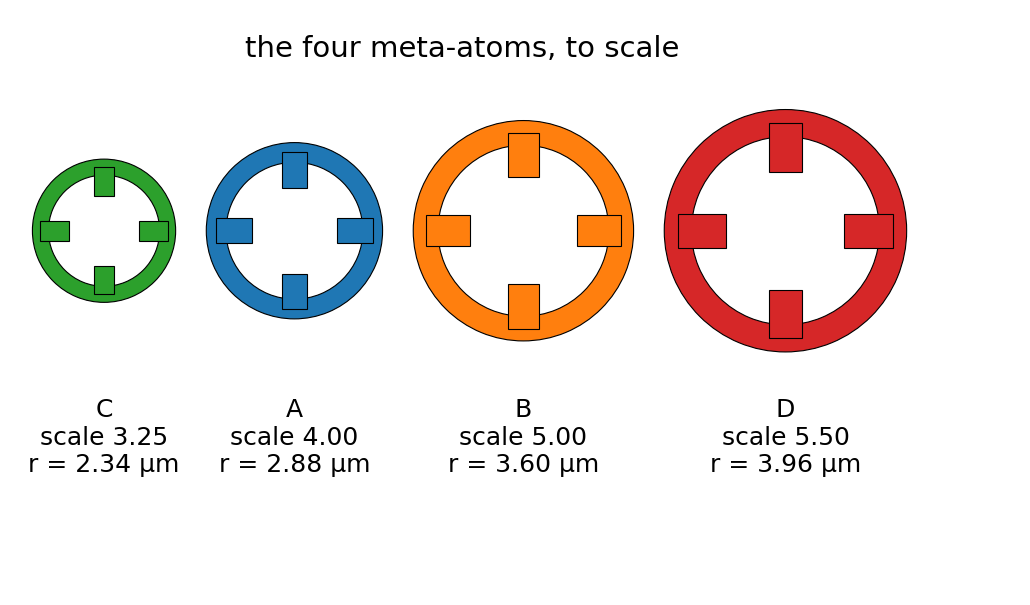
\includegraphics[width=0.72\textwidth]{figs/atoms_to_scale.png}
\caption{The four meta-atoms, drawn to scale. All are $0.2\um$-thick gold members
of the same parametric family, so their isolated resonances scale linearly with
the \code{scale} parameter (Table~\ref{tab:atoms}).}
\label{fig:atoms}
\end{figure}

\begin{table}[htbp]
\centering\small
\caption{The four measured meta-atoms. ``Residual'' and ``reciprocity'' are the
diagnostics stored in the \code{tmat.h5} files by the extraction; ``passivity''
is $\max \sigma(I + 2T)$, which should not exceed $1$. The isolated resonance
divided by \code{scale} is constant to $0.5\,\%$ across the family, which is the
evidence that no atom is anomalous.}
\label{tab:atoms}
\begin{tabular}{@{}lcccc@{}}
\toprule
 & \textbf{C} & \textbf{A} & \textbf{B} & \textbf{D} \\
\midrule
\code{scale} (3D Run ID)      & 3.25 (run 10) & 4.00 (run 6) & 5.00 (run 2) & 5.50 (run 3) \\
Ring outer radius $a$         & $2.338\um$ & $2.877\um$ & $3.596\um$ & $3.956\um$ \\
Stored \code{residual}        & 0.0045--0.0395 & 0.0024--0.0240 & 0.0039--0.0164 & 0.0045--0.0217 \\
Stored \code{reciprocity}     & 0.024--0.182 & 0.012--0.110 & 0.018--0.076 & 0.024--0.094 \\
Passivity, $\max \sigma(I+2T)$ & 1.037 & 1.028 & 1.021 & 1.049 \\
Isolated resonance / \code{scale} & 3.766 & 3.770 & 3.786 & 3.782 \\
\bottomrule
\end{tabular}
\end{table}

\subsection{The layouts}

All cells are $16\times16\um$ with four atoms on the $8\um$ square sub-lattice at
$(\pm 4, \pm 4)\um$, written $x,y;y,x$ for the two diagonals
(Fig.~\ref{fig:layouts}). This is \emph{not} simply a $2\times2$ tile: for a
two-species checkerboard both sublattices are square lattices of constant
$8\sqrt{2} = 11.31\um$ rotated by $45^\circ$, with one species at the body centre
of the other, so the true point group is $C_{4v}$ about one atom site. Filling the
four sites with four \emph{different} atoms removes that symmetry, and the $24$
assignments collapse under the $D_4$ symmetry of the site square to exactly three
distinct cells. All three were built and benchmarked.

\begin{figure}[htbp]
\centering
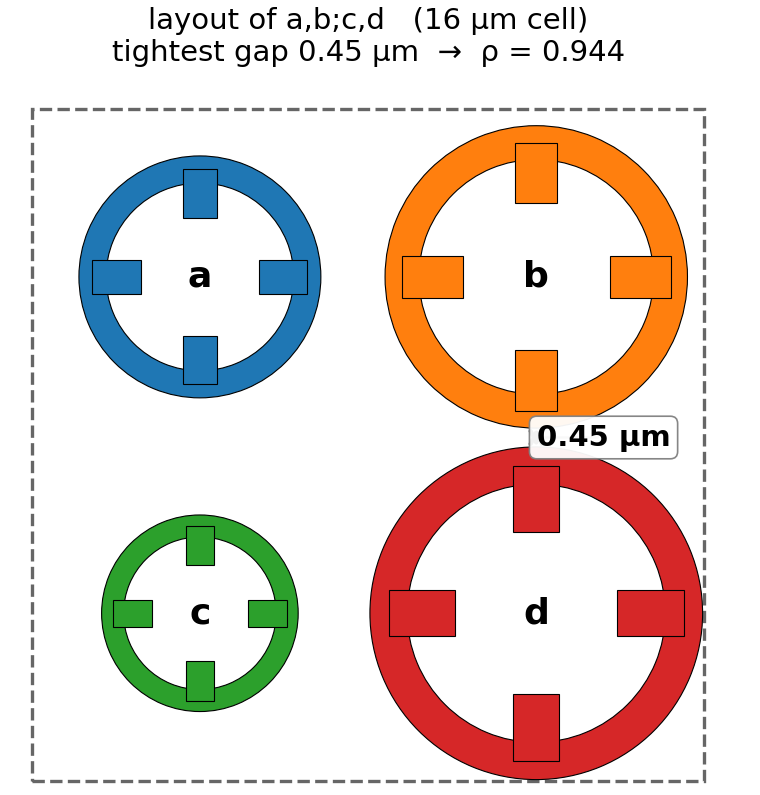
\includegraphics[width=0.31\textwidth]{figs/layout_abcd.png}\hfill
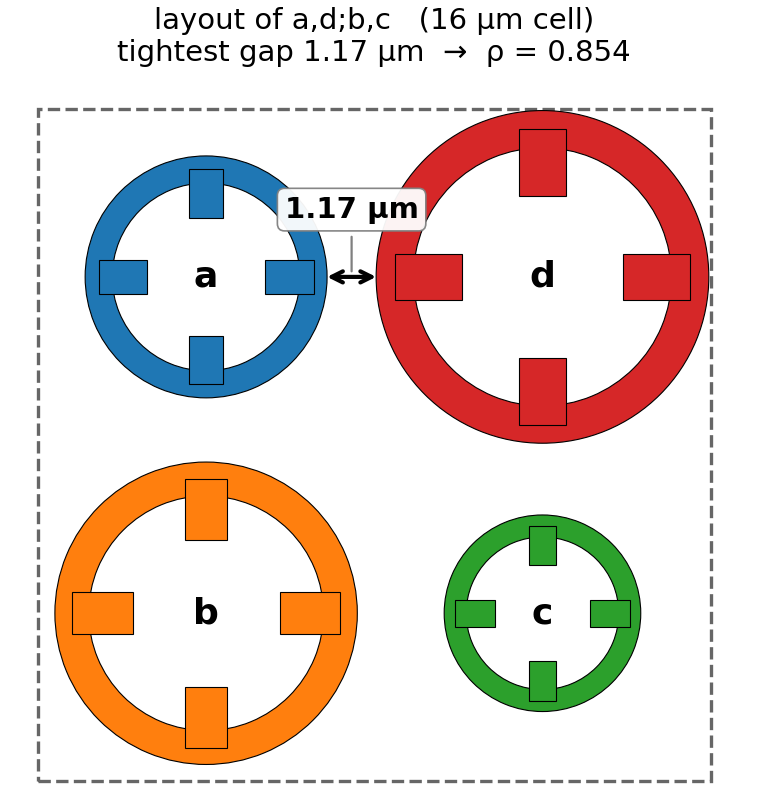
\includegraphics[width=0.31\textwidth]{figs/layout_adbc.png}\hfill
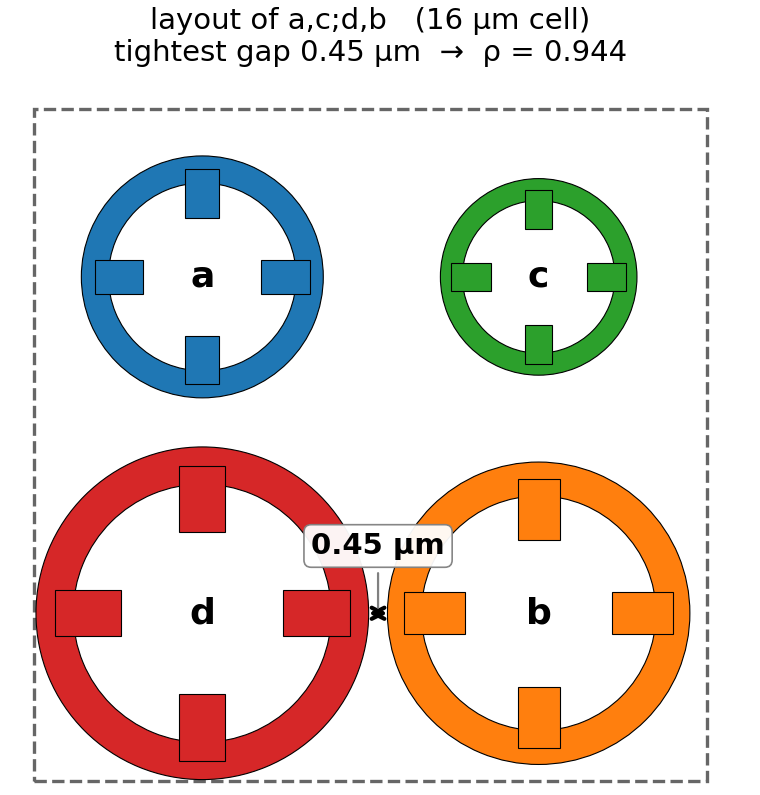
\includegraphics[width=0.31\textwidth]{figs/layout_acdb.png}
\caption{The three distinct four-species arrangements of the same four atoms on
the same lattice. Left, \texttt{a,b;c,d}: B and D adjacent, tightest gap
$0.45\um$, $\rho = 0.944$. Centre, \texttt{a,d;b,c}: B and D on a diagonal,
tightest gap $1.17\um$, $\rho = 0.854$. Right, \texttt{a,c;d,b}: B and D adjacent
again in a different symmetry class, $\rho = 0.944$. The right-hand cell is the
discriminating experiment of Section~\ref{sec:rho}.}
\label{fig:layouts}
\end{figure}

\subsection{The full-wave references}

Ten independent direct-CST periodic simulations serve as ground truth: four
single-species lattices (already available from the parametric sweep) and six
supercells. Each supercell run copies every solver, mesh, material and boundary
setting from the packed project's own periodic run, with $20$ Floquet modes per
port. A single \emph{empty-cell companion run} --- identical geometry, no metal
--- serves every cell: it measures the port-plane separation ($56.813\um$) and
doubles as the background test. Most supercells took about an hour on
$2$--$3$\,M tetrahedral DOF over $\sim\!48$ adaptive frequency points. The
four-atom cells are much heavier --- $4.2$\,M DOF and $1.8$\,h for
\texttt{a,b;c,d}, $1.7$\,h for \texttt{a,c;d,b}, and $6.4$\,M DOF and $4.9$\,h
for \texttt{a,d;b,c}, whose D-derived resonance sits on the $18.74\THz$ Rayleigh
edge.

%==============================================================================
\section{Validation of the implementation}
\label{sec:validation}
%==============================================================================

Before any comparison with full-wave, the aggregation was verified against
algebraic identities it must satisfy exactly, and against a wholly independent
implementation. Table~\ref{tab:identities} lists the results; all are round-off.

\begin{table}[htbp]
\centering\small
\caption{Internal consistency and independent cross-check. The \texttt{treams}
comparison is a second implementation of the \emph{whole chain} --- its own
cluster T-matrix, its own Ewald lattice interaction, its own plane-wave
projection with its own basis-position phases and power normalisation --- not
merely of the lattice sums. Forty such checks run in
\code{tests/aggregation/test\_supercell.py}.}
\label{tab:identities}
\begin{tabular}{@{}lr@{}}
\toprule
Identity or independent implementation & Residual \\
\midrule
$M = 1$ cell reduces to the one-atom code (coupling, $f$, $S_{11}/S_{21}$)
  & \textcolor{good}{bit-identical} \\
$2\times2$ cell of four identical atoms $\equiv$ the primitive lattice
  & \textcolor{good}{$\le 8\times10^{-16}$} \\
Basis-atom relabelling / whole-cell lattice shift
  & \textcolor{good}{$\le 7\times10^{-16}$ \,/\, $0$} \\
Checkerboard selection rule: power in the odd $(n_1{+}n_2)$ orders
  & \textcolor{good}{$\le 6\times10^{-33}$} \\
All $T = 0 \Rightarrow S = S_{\text{background}}$
  & \textcolor{good}{$0$} \\
Finite-cluster $T^{O}$ vs.\ the direct multi-centre far field, $L_C = 14$
  & \textcolor{good}{$1.9\times10^{-9}$} \\
Independent \texttt{treams} chain, every cell: complex $S_{21}$ \,/\, $S_{11}$
  & \textcolor{good}{$\le 3\times10^{-14}$ \,/\, $\le 1\times10^{-12}$} \\
\bottomrule
\end{tabular}
\end{table}

These results bound where any remaining error can live. They exclude coding
errors in the block solve, lattice-sum convergence, basis conventions and
normalisation, and the Floquet output map. Whatever disagreement with full-wave
survives must therefore live in what a truncated single-centre T-matrix can
\emph{represent}, or in the accuracy of the particular T-matrices supplied.

\begin{remark}[A trap in cross-code comparison]
Comparisons must match the incidence direction. Illuminating from $-z$ rather
than $+z$ changes the answer by $0.01$--$0.06$ in complex $S$ with these inputs
--- that is the input T-matrix's own up/down asymmetry, tracking its stored
\code{reciprocity} diagnostic, not an implementation difference. With matching
incidence the two codes agree to $10^{-12}$.
\end{remark}

%==============================================================================
\section{Results}
\label{sec:results}
%==============================================================================

\subsection{Single-species lattices}

Table~\ref{tab:step1} places each atom alone on its $8\um$ lattice against its own
direct CST run (Fig.~\ref{fig:singles}). The reconstruction reproduces the
lineshape, the depth and the full phase excursion in every case; what varies is
where the resonance sits.

\begin{table}[htbp]
\centering\small
\caption{Each atom alone on an $8\um$ square lattice against its own direct CST
run.}
\label{tab:step1}
\begin{tabular}{@{}lcccc@{}}
\toprule
 & A & B & C & D \\
\midrule
Transmission minimum, this pipeline & $13.039\um$ & $16.638\um$ & $10.897\um$ & $19.106\um$ \\
Transmission minimum, direct CST    & $13.126\um$ & $17.341\um$ & $10.933\um$ & $23.509\um$ \\
Resonance offset                    & $-0.66\,\%$ & $-4.05\,\%$ & $\mathbf{-0.33\,\%}$ & \textcolor{bad}{$\mathbf{-19\,\%}$} \\
Complex $S_{21}$, max / mean $|\Delta|$ & 0.062 / 0.030 & 0.121 / 0.054 & 0.035 / 0.017 & \textcolor{bad}{0.466 / 0.149} \\
Complex $S_{11}$, max / mean $|\Delta|$ & 0.065 / 0.041 & 0.135 / 0.073 & 0.040 / 0.020 & \textcolor{bad}{0.467 / 0.171} \\
Against the independent \texttt{treams} code & $\le 10^{-12}$ & $\le 10^{-12}$ & $\le 10^{-12}$ & $\le 10^{-12}$ \\
\bottomrule
\end{tabular}
\end{table}

\begin{figure}[htbp]
\centering
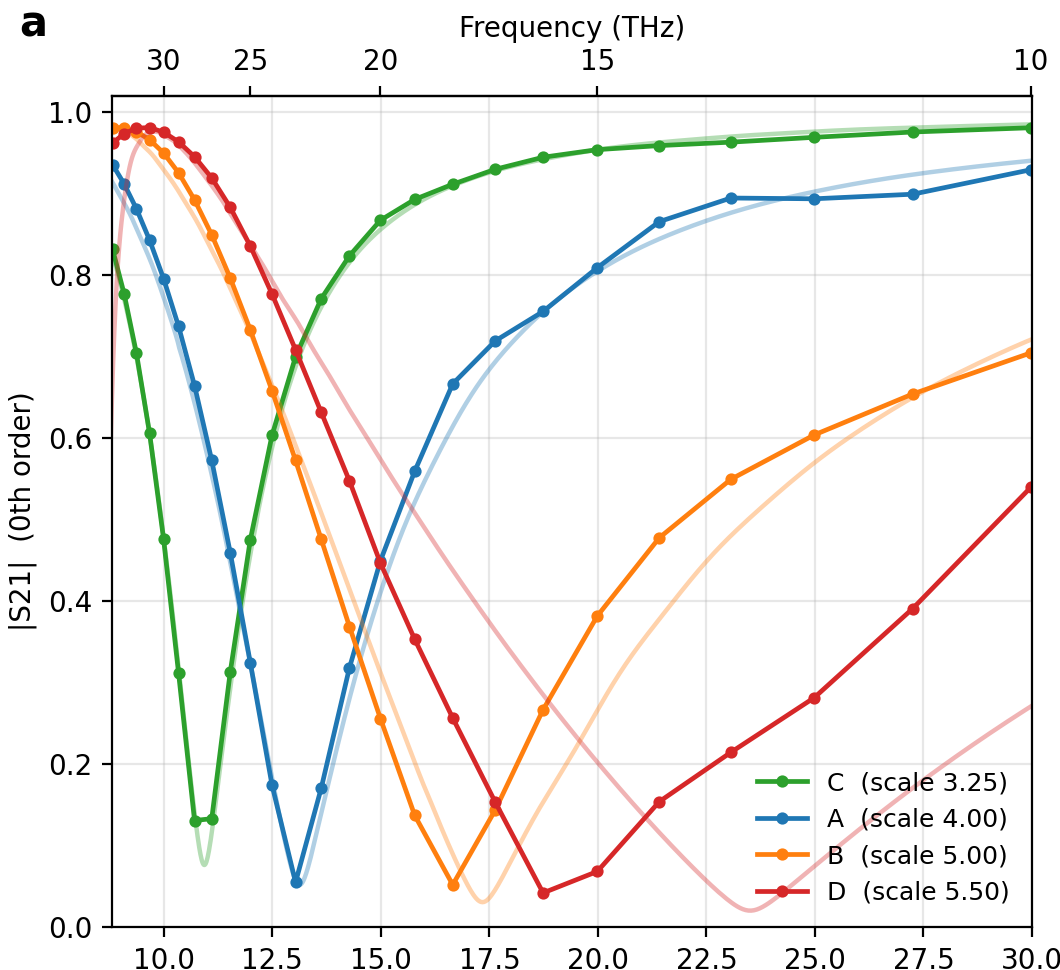
\includegraphics[width=0.62\textwidth]{figs/s21_singles.png}
\caption{One atom per $8\um$ cell: prediction (markers) against direct CST (pale
lines). C, A and B track closely; D, the largest, does not. Atom D's failure is
the most informative result in the study and is analysed in
Section~\ref{sec:Dalone}.}
\label{fig:singles}
\end{figure}

A subtlety worth extracting: \textbf{a file's worst diagnostic does not predict
its performance --- its quality \emph{at its own resonance} does.} Atom C has the
worst residual and the worst reciprocity in the whole set (to $0.040$ and
$0.18$, with passivity $1.037$) and reconstructs best, because those maxima sit at
$10$--$20\THz$ where C is a tiny, deeply-Rayleigh scatterer that barely
contributes, while at its own resonance the extraction is clean. Near a resonance
the Foldy--Lax denominator amplifies whatever error the input carries; far from
one it does not much matter.

\subsection{Two-species supercells: mixing is free}

A mixed cell is not an interpolation between its constituents. Every species
moves to a sparser $11.31\um$ sublattice and its resonance red-shifts --- by more
for the smaller, higher-frequency atom (Table~\ref{tab:shift}). Nevertheless,
every two-species mixed cell lands within the range of its two constituents
(Table~\ref{tab:mse}): \texttt{a,c;c,a}, from the pair that reconstructs best
individually, gives the best mixed cell; \texttt{a,b;b,a}, containing the worst
constituent, gives the worst.

\begin{table}[htbp]
\centering\small
\caption{Resonance of each species alone and in mixed cells. The shift is a
collective effect of the sparser sublattice, not an artefact.}
\label{tab:shift}
\begin{tabular}{@{}lcccc@{}}
\toprule
Resonance of & alone ($8\um$) & in \texttt{a,b;b,a} & in \texttt{a,c;c,a} & in \texttt{b,c;c,b} \\
\midrule
atom A & $13.04\um$ & 13.95 & 14.42 & --- \\
atom B & $16.64\um$ & 16.88 & --- & 16.71 \\
atom C & $10.90\um$ & --- & 11.84 & 12.44 \\
\bottomrule
\end{tabular}
\end{table}

\textbf{Dilution helps the worst atom.} Atom B's resonance is placed $4.05\,\%$
wrong on its own dense $8\um$ lattice; in a mixed cell, on the sparser
$11.31\um$ sublattice, the \emph{same} T-matrix places it to $+0.6\,\%$
(\texttt{a,b;b,a}) and $+0.44\,\%$ (\texttt{b,c;c,b}). The $4\,\%$ was never the
atom --- it was the strong collective shift of a dense lattice being computed
from a slightly wrong $T$. Halve the areal density and the lattice amplification
that produced it halves too.

\subsection{Collective physics the pipeline predicts, and full-wave confirms}
\label{sec:collective}

Three features appear only because the cell is a supercell. None is expressible
by a single-atom model, and each was predicted before being measured.

\paragraph{An exact selection rule.} For the two-species checkerboards, the
coherent basis sum of Eq.~\eqref{eq:floquet} extinguishes every order with
$n_1 + n_2$ odd, identically, whatever the two species are. The predicted power
in those channels is $\le 6\times10^{-31}$ across the band in all three cells (and $\le 2\times10^{-30}$ on the $4\times$ refined grids)
(the $6\times10^{-33}$ of Table~\ref{tab:identities} is the single validation
check at one frequency). CST measures $1.5\times10^{-5}$,
$1.5\times10^{-5}$ and $6.1\times10^{-6}$ against carriers of $0.987$, $1.002$
and $0.989$ --- the empty run's own noise floor --- over the entire
$18.7$--$34\THz$ window in which the channels are open. With four distinct atoms
the cancellation fails, the odd orders switch on, and the cells begin diffracting
$7.8\THz$ lower: CST measures $0.388$ against $0.409$ predicted for
\texttt{a,b;c,d}, and $0.403$ against $0.407$ for \texttt{a,c;d,b}.

\paragraph{A dark lattice resonance.} At $\lambda = 16.00\um$ --- the supercell's
own Rayleigh condition --- the near-field coupling $W_{st}$ becomes singular, but
the responsible channels carry no far field, by the same symmetry that makes them
dark. On a $4\times$ refined frequency grid every two-species cell shows it at
exactly the same place: $\mathrm{cond}(I - WT)$ peaks at $1302$, $594$ and $1198$
at $15.989\um$, with diffracted power $\sim\!10^{-30}$ and absorption rising to
$+0.349$, $+0.081$ and $+0.209$. The $8\um$ primitive lattice has no Rayleigh
onset until $8\um$ and shows nothing there at all. Direct CST confirms both the
darkness ($1.5\times10^{-5}$ against a $0.987$ carrier) and the associated
transmission window (predicted $15.57\um$ at $|S_{21}| = 0.68$; measured
$15.35\um$ at $0.72$). \emph{The feature's position depends only on the cell; its
strength depends on the contents.}

\paragraph{Arrangement as a design knob.} The three four-species cells contain
identical atoms on an identical lattice; $\sum_s T_s$ is the same for all three
and cannot tell them apart. Yet rearranging alone changes the complex $S_{21}$ by
up to $0.429$ (mean $0.159$) between \texttt{a,b;c,d} and \texttt{a,d;b,c}, and
the transmittance $|S_{21}|$ by up to $0.60$ across the three arrangements. The
cells also differ qualitatively: \texttt{a,b;c,d} is a
strong linear polariser near $18.7\um$ ($\max\bigl||t_{xx}| - |t_{yy}|\bigr| =
0.603$, mean $0.176$) while \texttt{a,d;b,c}, from the same four atoms, is nearly
isotropic ($0.168$, mean $0.037$). The two cells that put the two largest atoms
side by side are strongly birefringent; the one that puts them on a diagonal is
not. This is the sharpest statement in the study of why aggregation is a
multiple-scattering solve and not a sum of polarisabilities.

Cross-polarisation stays below $3.2\times10^{-12}$ in all three cells despite the
$C_1$ point group. This is an empirical cancellation tied to the square site
arrangement --- displacing one atom gives $|t_{xy}| = 10^{-2}$ --- for which no
symmetry argument is offered here (Section~\ref{sec:open}).

\subsection{The accuracy ordering}
\label{sec:ordering}

Table~\ref{tab:mse} scores all ten benchmarks by the mean squared error of the
complex specular $S_{21}$ against direct CST, on the complex amplitude so that a
phase error counts, and orders them by $\rho$ of Eq.~\eqref{eq:rho} taken over
the $8\um$ neighbour pairs. Figure~\ref{fig:mse} plots the same data.

\begin{table}[htbp]
\centering\small
\caption{All ten benchmarks, ordered by the addition-theorem convergence ratio
$\rho$. MSE is $\mathrm{mean}\,|S_{21}^{\text{pred}} - S_{21}^{\text{CST}}|^2$
over the stored frequencies. Seven of the ten land at mean $|\Delta S_{21}|$
$0.017$--$0.080$; three do not.}
\label{tab:mse}
\begin{tabular}{@{}lcccl@{}}
\toprule
Case & $\rho$ (worst pair) & MSE $S_{21}$ & mean $|\Delta S_{21}|$ & Verdict \\
\midrule
atom C alone      & 0.584 & 0.00038 & 0.017 & \textcolor{good}{good} \\
\texttt{a,c;c,a}  & 0.652 & 0.00067 & 0.019 & \textcolor{good}{good} \\
atom A alone      & 0.719 & 0.00107 & 0.030 & \textcolor{good}{good} \\
\texttt{b,c;c,b}  & 0.742 & 0.00171 & 0.036 & \textcolor{good}{good} \\
\texttt{a,b;b,a}  & 0.809 & 0.00367 & 0.046 & \textcolor{good}{good} \\
\texttt{a,d;b,c}  & 0.854 & 0.0118  & 0.080 & degrading \\
atom B alone      & 0.899 & 0.0039  & 0.054 & degrading \\
\texttt{a,c;d,b}  & 0.944 & 0.1207  & 0.244 & \textcolor{bad}{\textbf{broken}} \\
\texttt{a,b;c,d}  & 0.944 & \textbf{0.1654} & 0.308 & \textcolor{bad}{\textbf{broken}} \\
atom D alone      & 0.989 & 0.0351  & 0.149 & \textcolor{bad}{\textbf{broken}} \\
\bottomrule
\end{tabular}
\end{table}

\begin{figure}[htbp]
\centering
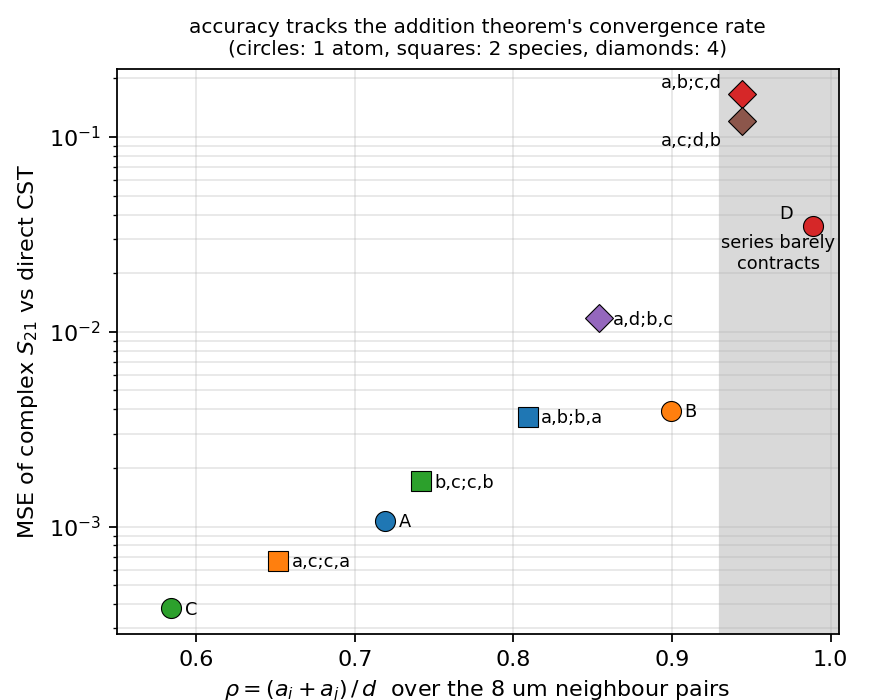
\includegraphics[width=0.60\textwidth]{figs/mse_vs_rho.png}
\caption{Accuracy against direct CST versus the convergence ratio $\rho$. Circles:
single-species lattices. Squares: two-species checkerboards. Diamonds:
four-species cells. Above $\rho \approx 0.94$ (shaded) the multipole series barely
contracts and the predictions break.}
\label{fig:mse}
\end{figure}

Two observations frame the rest of the paper. First, the ordering is strong:
below $\rho \approx 0.85$ every case is within the input T-matrices' own error,
and MSE separates the four-atom cells by $14\times$ ($0.1654$ against $0.0118$)
where mean absolute error separates them by only $3.8\times$, because the
\texttt{a,b;c,d} disagreement is concentrated in a few badly misplaced resonances
rather than spread across the band. Second, the ordering is not perfectly
monotone --- atom B alone beats \texttt{a,d;b,c}, and atom D alone beats
\texttt{a,b;c,d}. $\rho$ is therefore the right diagnostic for \emph{which regime
one is in}, not a quantitative error law.

%==============================================================================
\section{Failure analysis}
\label{sec:failure}
%==============================================================================

\subsection{Case study 1: the \texttt{a,b;c,d} supercell}
\label{sec:abcd}

\texttt{a,b;c,d} and \texttt{a,d;b,c} contain the same four atoms on the same
$16\um$ lattice with the same $8\um$ sub-lattice. They differ only in which atoms
end up adjacent. The accuracy differs by $14\times$ (Fig.~\ref{fig:abcd}).

\begin{figure}[htbp]
\centering
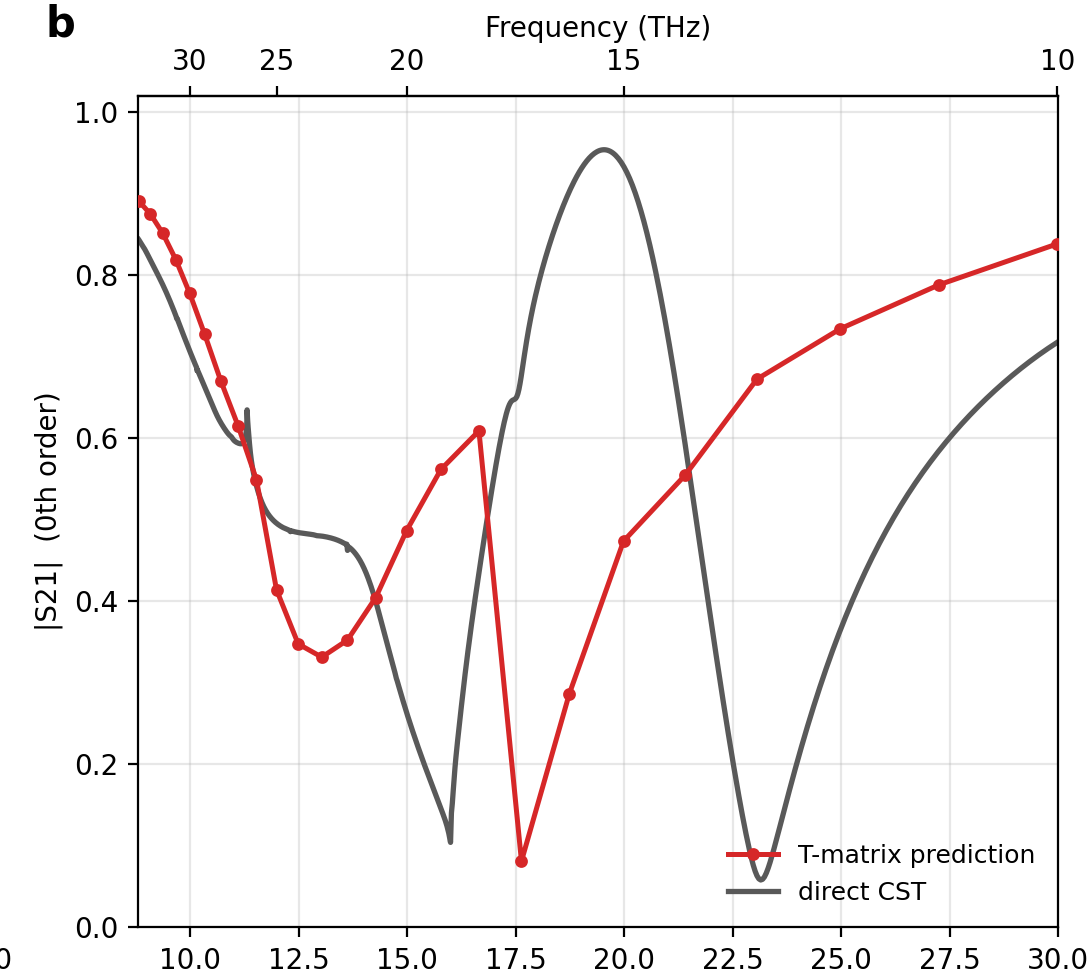
\includegraphics[width=0.47\textwidth]{figs/s21_abcd_vs_cst.png}\hfill
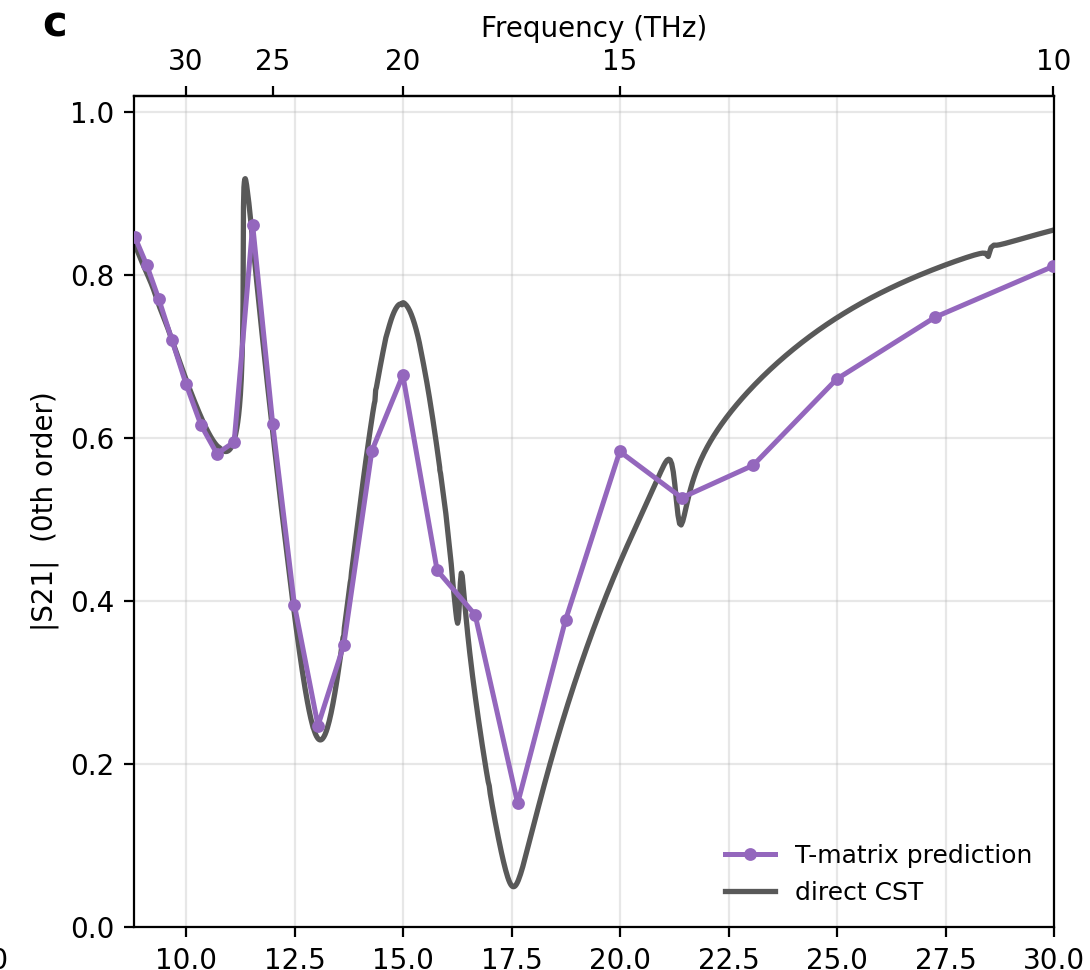
\includegraphics[width=0.47\textwidth]{figs/s21_adbc_vs_cst.png}
\caption{Left, \texttt{a,b;c,d} ($\rho = 0.944$): the deepest transmission dip is
misplaced by $-5.51\um$ and the whole mid-band structure is wrong. Right,
\texttt{a,d;b,c} ($\rho = 0.854$): the same four atoms on the same lattice,
re-paired, tracking full-wave. Grey: direct CST.}
\label{fig:abcd}
\end{figure}

The worst neighbour pair in \texttt{a,b;c,d} is B--D: $a_B + a_D = 3.596 + 3.956
= 7.552\um$ against $d = 8\um$, a metal-to-metal gap of $0.448\um$ and $\rho =
0.944$. Re-pairing to put A--D adjacent gives $\rho = 0.854$.

Two features of the failure matter for what follows. It is \textbf{not a
calibratable bias}: \texttt{a,b;c,d} and its $\rho$-twin \texttt{a,c;d,b}
misplace their deepest dip by $-5.51\um$ and $+4.92\um$ respectively --- opposite
signs. And it is \textbf{channel-selective}: the total diffracted power of
\texttt{a,b;c,d} is predicted at $0.409$ against $0.388$ measured
($5.4\,\%$ relative), and its $\rho$-twin keeps $1.0\,\%$ ($0.407$ against
$0.403$), so the specular channel breaks well before the diffracted ones.

\subsection{Case study 2: atom D's own lattice}
\label{sec:Dalone}

Atom D alone on its $8\um$ lattice places its array resonance at $19.1\um$
against $23.5\um$ measured --- a $19\,\%$ error --- and drives the computed
absorption negative (Fig.~\ref{fig:Dalone}).

\begin{figure}[htbp]
\centering
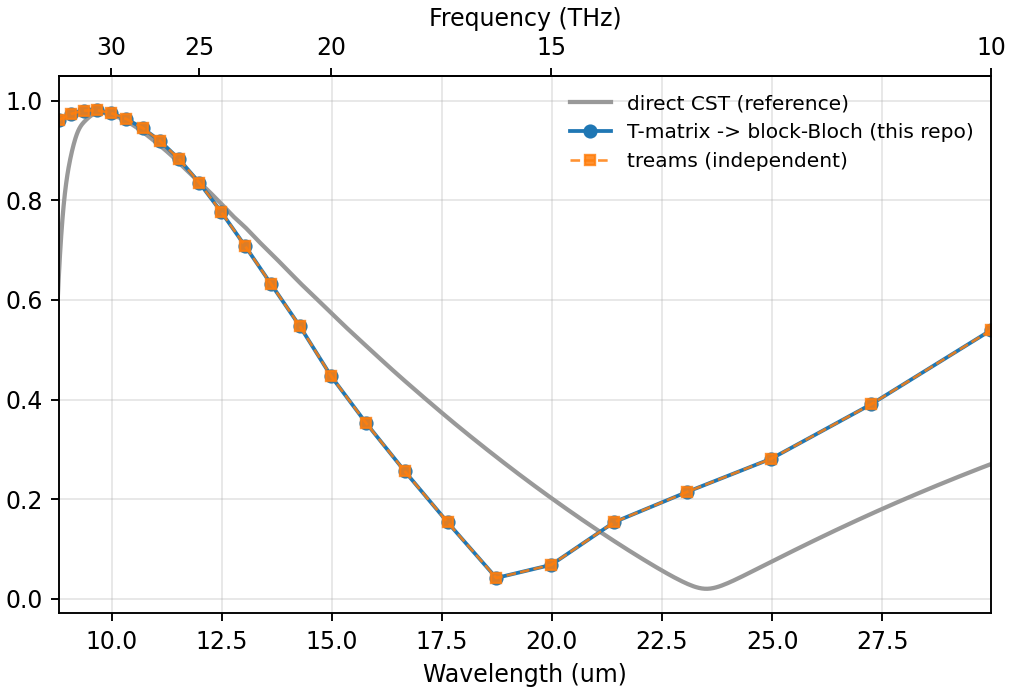
\includegraphics[width=0.62\textwidth]{figs/s21_D_alone.png}
\caption{Atom D alone on its $8\um$ lattice. This package (blue) and
\texttt{treams} (orange) are indistinguishable; both sit far from direct CST
(grey). Predicted dip $19.1\um$ against $23.5\um$ measured.}
\label{fig:Dalone}
\end{figure}

The direction of the error is the clue. A, B and C all \emph{blue}-shift from
their isolated resonance to their $8\um$ array resonance by a consistent
$1.3$--$2.0\um$. D \emph{red}-shifts by $+2.74\um$. Across the parametric sweep,
array-dip/\code{scale} is flat at $\approx 3.3$ while the neighbours are far
apart and then climbs sharply as the gap closes:

\begin{center}\small
\begin{tabular}{@{}cccc@{}}
\toprule
\code{scale} & Gap between neighbours & CST array dip & dip / \code{scale} \\
\midrule
4.00 & $2.246\um$ & $13.13\um$ & 3.283 \\
4.50 & $1.526\um$ & $14.90\um$ & 3.311 \\
5.00 & $0.807\um$ & $17.34\um$ & 3.468 \\
\textbf{5.50 (= D)} & $\mathbf{0.088\um}$ & $\mathbf{23.51\um}$ & $\mathbf{4.275}$ \\
\bottomrule
\end{tabular}
\end{center}

At \code{scale} $5.5$ the rings are $88$\,nm apart. This is the classic
near-touching capacitive red-shift: a hybridised gap mode of the pair, real
physics in the full-wave model, and the same effect that already makes atom B
$4\,\%$ off while atom A is $0.7\,\%$.

\subsection{Eliminating the alternatives}

\paragraph{The T-matrix is innocent.} Asking each extracted $T$ where its own
\emph{isolated} atom resonates gives a perfectly linear size scaling:
peak/\code{scale} $= 3.766, 3.770, 3.786, 3.782$ for C, A, B, D
(Table~\ref{tab:atoms}). D's T-matrix is fully consistent with its siblings.
It is also the most dipolar of the four ($96.5\,\%$ $l = 1$), so truncating
\emph{its own} multipole content is not the issue --- and raising $\lmax$ makes
the result worse, not better.

\paragraph{The implementation is innocent.} \texttt{treams} reproduces atom D's
reconstruction to $1.2\times10^{-15}$ (Fig.~\ref{fig:crosscode}) because it
evaluates the same addition theorem at the same $\lmax$ and inherits the same
convergence limit. This is the sharpest demonstration in the study that
\emph{cross-code agreement validates the implementation and only full-wave
validates the physics}.

\begin{figure}[htbp]
\centering
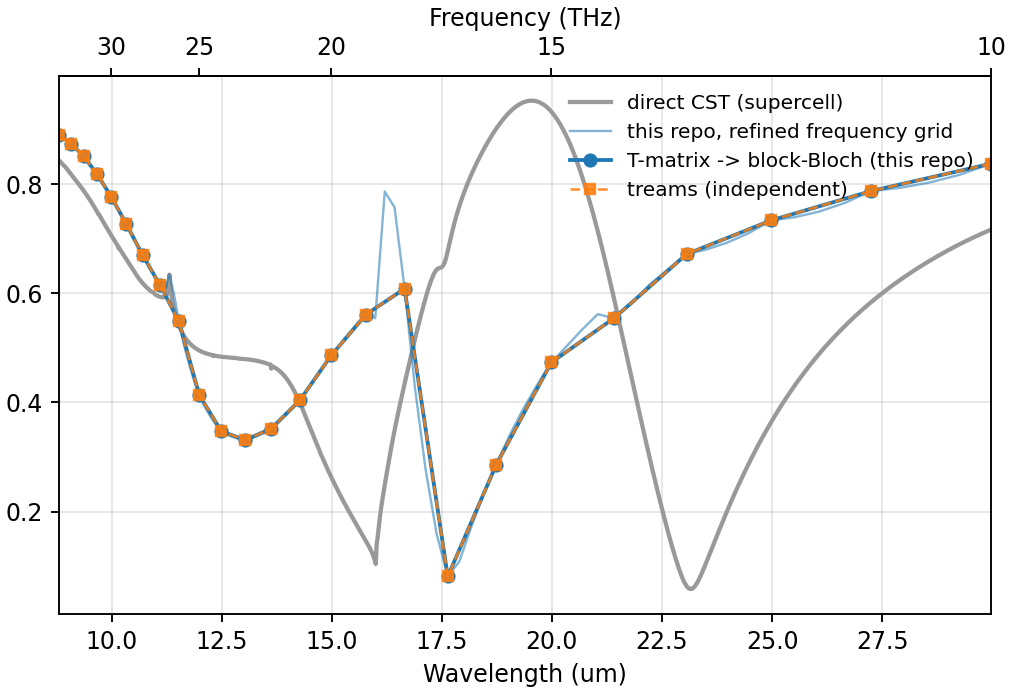
\includegraphics[width=0.72\textwidth]{figs/s21_abcd_full.png}
\caption{\texttt{a,b;c,d}, complex $S_{21}$ and $S_{11}$. This package (blue) and
the independent \texttt{treams} implementation (orange) are indistinguishable at
$10^{-14}$ --- and both sit far from direct CST (grey). Thin blue line: the same
prediction on a refined frequency grid.}
\label{fig:crosscode}
\end{figure}

\paragraph{Arrangement symmetry is not the driver.} In the two four-atom cells
originally available, $\rho$ was confounded with how nearly mirror-symmetric the
arrangement was, because putting the two largest atoms on a diagonal does both at
once. A third cell, \texttt{a,c;d,b}, was built specifically to separate them: it
reproduces \texttt{a,b;c,d}'s worst pair, its $\rho = 0.944$ and its $0.448\um$
gap exactly, while placing a different pair on the diagonal. It lands with
\texttt{a,b;c,d} ($0.1207$ against $0.1654$), not with \texttt{a,d;b,c}
($0.0118$). The two cells sharing $\rho = 0.944$ are within $1.4\times$ of each
other; the cell at $\rho = 0.854$ is $10$--$14\times$ better than either.

\subsection{The mechanism}
\label{sec:rho}

What fails is neither the T-matrix, nor the lattice sum, nor the solver, but the
\emph{truncation} of the addition theorem~\eqref{eq:addition}.

The validity condition~\eqref{eq:validity} is \emph{satisfied} in every case in
this study --- even D--D at $8\um$, where $a_i + a_j = 7.912\um$ against $8.000$.
Nothing is formally invalid; no assertion fires; no matrix is singular. What
varies is the rate. With truncation error $\sim \rho^{\lmax}$, the multipole
order required for a $1\,\%$ coupling error is $\ln(0.01)/\ln\rho$:

\begin{center}\small
\begin{tabular}{@{}clcc@{}}
\toprule
$\rho$ & Case & Error factor per extra order & $\lmax$ for $\sim\!1\,\%$ \\
\midrule
0.652 & \texttt{a,c;c,a} & $\times 0.65$ & 11 \\
0.809 & \texttt{a,b;b,a} & $\times 0.81$ & 22 \\
\textcolor{bad}{0.944} & \textcolor{bad}{\texttt{a,b;c,d} (B--D pair)} & \textcolor{bad}{$\times 0.94$} & \textcolor{bad}{\textbf{80}} \\
\textcolor{bad}{0.989} & \textcolor{bad}{atom D alone (D--D pair)} & \textcolor{bad}{$\times 0.99$} & \textcolor{bad}{\textbf{416}} \\
\bottomrule
\end{tabular}
\end{center}

\noindent
All runs use $\lmax = 3$. Physically: the field in a $0.448\um$ gap between two
$4\um$ objects varies on the scale of the gap, and spherical harmonics centred
$8\um$ away are a poor basis for it. \emph{Marginally satisfied is, in practice,
worse than violated, because nothing warns you.}

\subsection{Why raising the multipole order does not help}
\label{sec:lmax}

The obvious response --- increase $\lmax$ --- fails because two errors move in
opposite directions.

\begin{itemize}[leftmargin=*,itemsep=2pt]
\item \textbf{Truncation error falls} like $\rho^{\lmax}$, requiring
      $\lmax \approx 80$ for the B--D pair.
\item \textbf{Noise amplification rises.} The $l = 4, 5$ rows of these measured
      T-matrices sit at the extraction noise floor, and the near-field lattice sum
      amplifies exactly those rows. With $h^{(1)}_l(kp) \sim
      (2l-1)!!/(kp)^{\,l+1}$ and $kp$ falling from $5.70$ to $1.68$ across the
      band, $|W|$ at $l = 3$ reaches $1025$ at $\lambda \approx 30\um$ against
      $1.7$ at $8.82\um$ --- at the long-wavelength end the $l = 3$ coupling is
      $227\times$ the dipole coupling at the same frequency.
\end{itemize}

Both are measured, not predicted. Atom D's reconstruction is \emph{worse} at
$\lmax = 5$ than at $\lmax = 3$: the noise term already dominates before the
truncation term has begun to contract.

This also removes the natural internal diagnostic. An invalid translation ought
to fail to converge in multipole order, so an $\lmax\!=\!3\to4\to5$ spread should
flag the bad cells. It does not: \texttt{a,d;b,c} --- the widest gap and the best
CST agreement of the four-atom cells --- has the \emph{largest} spread, because
the spread mostly measures noise amplification rather than geometry.

%==============================================================================
\section{The limitation, and why it cannot be repaired in the aggregation}
\label{sec:limit}
%==============================================================================

\subsection{Statement}

\begin{quote}
\itshape
For two scatterers whose circumscribing spheres nearly touch, the multipole order
required to couple them accurately grows as $\ln\varepsilon / \ln\rho$. A stored
single-centre T-matrix band-limited to $l \le L$ contains neither the object's
response to, nor its emission into, the channels that carry the gap-scale field.
The deficiency is one of representation, and $\rho$ is fixed by geometry ---
circumscribing radii and centre distance --- not by any choice the solver makes.
\end{quote}

\subsection{Improving the inter-atom coupling cannot help}
\label{sec:proof}

It is natural to suppose that the cure lies in computing the lattice coupling
more accurately, or to higher order. It does not, and the reason is structural.

\begin{proposition}[Band-limitation of the multiple-scattering solution]
\label{prop:sandwich}
Let $\Pi$ be the orthogonal projector onto the modes with $l \le L$, and suppose
every stored transition matrix is band-limited, $T = \Pi T \Pi$. Then the solution
$f = T(I - WT)^{-1}a_{\text{inc}}$ of Eq.~\eqref{eq:foldy} depends on the lattice
coupling operator $W$ only through its block $\Pi W \Pi$, and on the incident vector
only through $\Pi a_{\text{inc}}$.
\end{proposition}

\begin{proof}
Let $v = (I - WT)^{-1}a_{\text{inc}}$, so that
$v = a_{\text{inc}} + W T v$ and $f = Tv$. Because $T = \Pi T \Pi$ we have $T = T\Pi =
\Pi T$, hence $f = Tv = \Pi T(\Pi v)$: the output lies in $\operatorname{ran}\Pi$ and is
determined by $\Pi v$ alone. Projecting the fixed-point equation,
\begin{equation*}
  \Pi v \;=\; \Pi a_{\text{inc}} + \Pi W T v
      \;=\; \Pi a_{\text{inc}} + \Pi W (\Pi T \Pi) v
      \;=\; \Pi a_{\text{inc}} + (\Pi W \Pi)\,T\,(\Pi v),
\end{equation*}
where the last step is associativity together with $T = \Pi T \Pi$. Writing $w = \Pi v$,
\begin{equation}
  \bigl(I - (\Pi W \Pi)T\bigr)\,w \;=\; \Pi a_{\text{inc}},
  \qquad
  f = T w .
  \label{eq:projected}
\end{equation}

It remains to check that Eq.~\eqref{eq:projected} \emph{determines} $w$, i.e.\
that $I - (\Pi W \Pi)T$ is invertible on $\operatorname{ran}\Pi$; otherwise the projected
system would have a solution manifold and the choice among its members could
still depend on the discarded part of $W$. Note first that $(\Pi W \Pi)T = \Pi W T$, since
$\Pi T = T$. Suppose $w \in \operatorname{ran}\Pi$ satisfies $(I - \Pi W T)w = 0$, and set
$v = w + (I - \Pi)WTw$. Then
\begin{equation*}
  (I - WT)v = w + (I-\Pi)WTw - WT\bigl(w + (I-\Pi)WTw\bigr) = w - \Pi W Tw = 0,
\end{equation*}
using $T(I-\Pi) = 0$. Invertibility of $I - WT$ gives $v = 0$, hence $w = \Pi v = 0$.
So $I - \Pi W T$ is injective on the finite-dimensional space
$\operatorname{ran}\Pi$, therefore invertible there, and $w$ --- and with it $f$ ---
is a function of $\Pi W \Pi$ and $\Pi a_{\text{inc}}$ alone.
\end{proof}

\noindent
Two features of the argument matter. It nowhere assumes the Neumann series
converges: it is an identity of the resolvent, valid whenever $(I - WT)$ is
invertible --- including next to the collective resonances where
$\mathrm{cond}(I - WT)$ reaches $1302$ (Section~\ref{sec:collective}). And it
places no hypothesis on $a_{\text{inc}}$, which is what makes the following
corollary work.

\begin{corollary}
\label{cor:padding}
Work in an enlarged basis of order $L' > L$, computing $W$ there by any method
that reproduces the exact translation coefficients on the $l \le L$ block ---
Ewald summation, an exact real-space sum, an analytic formula, or any future
method with that property --- and padding the stored $T$ with exact zeros outside
its $l \le L$ block. Then the predicted S-parameters are unchanged.
\end{corollary}

\begin{proof}
The padded $T$ satisfies $T = \Pi_L T \Pi_L$, so Proposition~\ref{prop:sandwich}
applies with $\Pi = \Pi_L$, \emph{provided} $I - W'T'$ is invertible in the enlarged
space. It is: if $(I - W'T')v = 0$ then $\Pi_L v = (\Pi_L W' \Pi_L) T' (\Pi_L v) =
W T (\Pi_L v)$, so invertibility of $I - WT$ on the order-$L$ space gives
$\Pi_L v = 0$, hence $T'v = T' \Pi_L v = 0$ and $v = W'T'v = 0$; finite
dimensionality does the rest. The proposition then says the solution depends only
on $\Pi_L W' \Pi_L$ --- which by hypothesis is the $W$ already in use --- and on
$\Pi_L a_{\text{inc}}$, which is the original incident vector. Note that the plane
wave \emph{does} have genuinely nonzero coefficients for $L < l \le L'$; absorbing
them is exactly what the proposition's freedom in $a_{\text{inc}}$ buys. The
scattered vector $f$ is therefore unchanged, and the Floquet
map~\eqref{eq:floquet} is an exact functional of $f$.
\end{proof}

Equivalently, in the Neumann expansion
$f = Ta + TWTa + TWTWTa + \cdots$, every occurrence of $W$ is sandwiched between
two copies of $T$, and its high-$l$ rows and columns are annihilated on contact.
The padding must be with exact zeros: extrapolating a physically motivated
high-$l$ tail is not padding but a change of $T$, and is precisely the (legitimate)
move Section~\ref{sec:multicentre} makes.

Note also what the sandwich argument does \emph{not} reach. It applies to the
periodic solve of Eq.~\eqref{eq:foldy}, where every $W$ sits between two $T$'s.
It does not apply to the finite-cluster operator of Eq.~\eqref{eq:cluster},
$T^{O} = Q(I - TU)^{-1}TP$, whose outward map $Q$ multiplies from the left and
inward map $P$ from the right: their high-$l$ rows and columns are unsandwiched
and do change the answer. That is exactly why the cluster order $L_C$ matters
there, improving $T^{O}$ from $1.7\times10^{-7}$ at $L_C = 12$ to
$1.9\times10^{-9}$ at $L_C = 14$ (Section~\ref{sec:theory}).

The argument that closes off the aggregation therefore has two parts, and it is
worth separating them, because Proposition~\ref{prop:sandwich} alone does not
close it. \emph{(a)} Proposition~\ref{prop:sandwich} confines whatever the
aggregation can contribute to the block $\Pi W \Pi$: anything outside it is inert.
\emph{(b)} That block is a measured quantity, and it is already exact --- the
Ewald sum of Section~\ref{sec:taper} agrees with an independent implementation to
$10^{-14}$, with an $\eta$-stability bracket to confirm it. There is nothing left
inside $\Pi W \Pi$ to gain and nothing outside it that matters.

The distinction is not pedantic: a modification that \emph{changes} $\Pi W \Pi$ does
change the answer, and Section~\ref{sec:taper} is exactly such a case ---
replacing the tapered real-space sum by Ewald moved the per-block error from
$4\times10^{-2}$ to $10^{-14}$ and is what made the heterogeneous cells correct
at all. What is closed off is further accuracy in an operator that is already
converged, not the operator's identity. The information deficit is in $T$.

\subsection{Merging the near-touching pair fails on geometry}
\label{sec:merge}

The other intuitive remedy --- treat the near-touching pair as one object,
extracted together, so that the gap lies \emph{inside} the new circumscribing
sphere --- is sound in principle and unavailable here. The minimal enclosing
sphere of two balls of radii $a_s, a_t$ at separation $d$ (neither containing the
other) has radius
\begin{equation}
  R = \frac{d + a_s + a_t}{2},
  \label{eq:mergeR}
\end{equation}
at distance $(d + a_t - a_s)/2$ from the centre of the ball of radius $a_s$, i.e.\
shifted towards the \emph{larger} ball. For $d = 8\um$
that is $R \approx 7$--$8\um$, which then overlaps the remaining atoms of the
densely packed cell:

\begin{center}\small
\begin{tabular}{@{}lccl@{}}
\toprule
Merge & Merged radius $R$ & Worst $\rho$ vs.\ the rest & Status \\
\midrule
B $+$ D & $7.776\um$ & 1.180 & \textcolor{bad}{violates Eq.~\eqref{eq:validity}} \\
A $+$ B & $7.237\um$ & 1.273 & \textcolor{bad}{violates Eq.~\eqref{eq:validity}} \\
C $+$ D & $7.147\um$ & 1.247 & \textcolor{bad}{violates Eq.~\eqref{eq:validity}} \\
\bottomrule
\end{tabular}
\end{center}

\noindent
(Worst $\rho$ computed from the shifted centre of Eq.~\eqref{eq:mergeR} over all
remaining atoms and all periodic images; the nearest image ties the nearest
in-cell atom in every row and changes nothing.) Merging all four is simply direct
simulation of the supercell, which forfeits the entire method. Merging therefore
helps only in sparse cells --- and these cells are not sparse.

\subsection{What must change: a distributed multi-centre representation}
\label{sec:multicentre}

The one change that restores convergence is to stop describing each atom by a
single expansion centre with a $\sim\!4\um$ circumscribing sphere, and describe
it instead by many small centres. The validity region then becomes the
\emph{union} of small spheres rather than one large one, and the pair convergence
ratio for the closest sub-centres across a physical gap $g$ becomes
\begin{equation}
  \rho_{\text{sub}} = \frac{2 r_s}{g + 2 r_s} ,
  \label{eq:rhosub}
\end{equation}
which can be driven as low as desired by shrinking the sub-centre radius $r_s$.
The gap $g$ is fixed by physics; $\rho$ is not (Fig.~\ref{fig:multicentre}).

\begin{figure}[htbp]
\centering
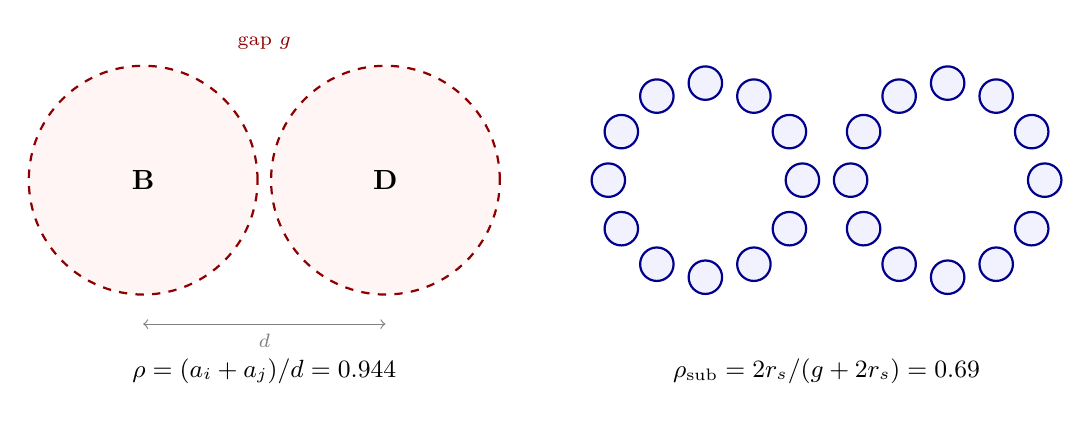
\begin{tikzpicture}[scale=0.85]
  % --- left: single-centre, near-touching
  \begin{scope}[shift={(0,0)}]
    \draw[dashed,thick,red!55!black,fill=red!4] (0,0) circle (1.709);
    \draw[dashed,thick,red!55!black,fill=red!4] (3.62,0) circle (1.709);
    \node at (0,0) {\bfseries B};
    \node at (3.62,0) {\bfseries D};
    \draw[<->,gray] (0,-2.15) -- node[below,font=\scriptsize]{$d$} (3.62,-2.15);
    \node[font=\scriptsize,red!55!black] at (1.81,2.05) {gap $g$};
    \node[font=\small] at (1.81,-2.85) {$\rho = (a_i+a_j)/d = 0.944$};
  \end{scope}
  % --- right: multi-centre
  \begin{scope}[shift={(8.4,0)}]
    \foreach \k in {0,...,11}{
      \draw[thick,blue!55!black,fill=blue!5]
        ({1.45*cos(\k*30)},{1.45*sin(\k*30)}) circle (0.25);}
    \foreach \k in {0,...,11}{
      \draw[thick,blue!55!black,fill=blue!5]
        ({3.62+1.45*cos(\k*30)},{1.45*sin(\k*30)}) circle (0.25);}
    \node[font=\small] at (1.81,-2.85) {$\rho_{\text{sub}} = 2r_s/(g+2r_s) = 0.69$};
  \end{scope}
\end{tikzpicture}
\caption{Left: the single-centre representation. Each T-matrix is valid only
outside its dashed circumscribing sphere, and for a sub-micron gap the two
spheres nearly touch, so $\rho \to 1$. Right: the distributed representation.
Covering the same object with sub-centres of radius $r_s$ makes the convergence
ratio a design parameter, Eq.~\eqref{eq:rhosub}. The gap $g$ is unchanged; only
the representation is.}
\label{fig:multicentre}
\end{figure}

\begin{table}[htbp]
\centering\small
\caption{Effect of a distributed representation on the three critical pairs, at
a uniform sub-centre radius $r_s = 0.5\um$. The last column inverts
Eq.~\eqref{eq:rhosub} for a target ratio. Note that $\rho_{\text{sub}}$ must be
compared with $\rho$ \emph{at equal sub-centre order}: the accuracy proxy is
$\rho^{\lmax}$, not $\rho$, and Table~\ref{tab:cost} does that comparison
properly.}
\label{tab:rhosub}
\begin{tabular}{@{}lcccc@{}}
\toprule
Pair & Gap $g$ & $\rho$ today & $\rho_{\text{sub}}$ at $r_s = 0.5\um$ & $r_s$ for $\rho_{\text{sub}} \le 0.75$ \\
\midrule
B--D & $0.448\um$ & 0.944 & \textcolor{good}{\textbf{0.691}} & $\le 0.672\um$ \\
A--D & $1.167\um$ & 0.854 & \textcolor{good}{0.461} & $\le 1.751\um$ \\
D--D & $0.088\um$ & 0.989 & 0.919 & $\le 0.132\um$ \\
\bottomrule
\end{tabular}
\end{table}

\paragraph{Sizing the change honestly.} It is tempting to argue that because
$k r_s = 0.23$ at the band centre for $r_s = 0.5\um$, each sub-centre is deeply
subwavelength and needs only dipoles. \emph{That argument is the very fallacy
this paper diagnoses.} A small $k r_s$ measures the sub-sphere against the
\emph{wavelength}; the binding comparison is against the \emph{gap}, and
$2 r_s = 1.0\um$ is more than twice the B--D gap of $0.448\um$. The correct
criterion is the accuracy proxy $\rho_{\text{sub}}^{\lmaxs}$ of
Eq.~\eqref{eq:rate}, applied at the sub-centre order $\lmaxs$.

Calibrating against the best-behaved benchmark in the study --- \texttt{a,c;c,a},
at $\rho = 0.652$ and $\lmax = 3$, hence $\rho^{\lmax} = 0.277$ --- and taking
$N_c \ge \pi(a - r_s)/r_s$ sub-centres of $2\lmaxs(\lmaxs + 2)$ modes each
gives the trade-off in Table~\ref{tab:cost}. It is non-monotone: shrinking $r_s$
lowers the order required but raises the centre count, so an interior optimum
exists.

\begin{table}[htbp]
\centering\small
\caption{Cost of the distributed representation at equal accuracy proxy
($\rho_{\text{sub}}^{\lmaxs} \le 0.277$), for a ring of outer radius
$a = 3.956\um$. For each sub-centre order $\lmaxs$ the cheapest admissible radius
is the largest one, $r_s^\star = \rho^\star g / [2(1-\rho^\star)]$ with
$\rho^\star = 0.277^{1/\lmaxs}$; the rows tabulate those. The single-centre
baseline is $30$ modes per atom. \textbf{Bold} marks the minimum over $r_s$,
which falls at $\lmaxs = 2$ for both pairs.}
\label{tab:cost}
\begin{tabular}{@{}lccccr@{}}
\toprule
Pair (gap) & $r_s$ & $\rho_{\text{sub}}$ & $\lmaxs$ & $N_c$ & Modes / atom \\
\midrule
B--D ($0.448\um$) & $0.086\um$ & 0.277 & 1 & 142 & 852 \\
                  & $\mathbf{0.249\um}$ & \textbf{0.527} & \textbf{2} & \textbf{47} & \textcolor{good}{\textbf{752}} \\
                  & $0.420\um$ & 0.652 & 3 & 27  & 810 \\
                  & $0.592\um$ & 0.726 & 4 & 18  & 864 \\
\midrule
D--D ($0.088\um$) & $0.017\um$ & 0.277 & 1 & 734 & 4404 \\
                  & $\mathbf{0.049\um}$ & \textbf{0.527} & \textbf{2} & \textbf{251} & \textcolor{good}{\textbf{4016}} \\
                  & $0.082\um$ & 0.652 & 3 & 148 & 4440 \\
                  & $0.116\um$ & 0.726 & 4 & 104 & 4992 \\
\bottomrule
\end{tabular}
\end{table}

The optimum sits at $\lmaxs = 2$ for both pairs, at the same
$\rho_{\text{sub}} = 0.527$ --- neither pure dipoles nor the single-centre order,
but the balance between them. The realistic figure is therefore
$752$ modes per atom for the B--D pair --- $25\times$ today's $30$, not the
$6\times$ a dipoles-only argument would suggest --- and $4016$ for the extreme
D--D geometry. The \emph{solve} remains comfortable: a four-atom cell at $752$
modes per atom is a $3008 \times 3008$ dense system, seconds of work. The \emph{extraction} is where
the cost lands, and Section~\ref{sec:aggchange} takes that up.

Two refinements reduce the figures above and are not included in them. A
\emph{graded} decomposition exploits the fact that the condition
$r_p + r_q < d_{pq}$ is per sub-pair: small spheres are needed only on the arcs
facing a close neighbour, while the far side of each ring stays coarse. And the
sub-centres need cover only the metal, not the circumscribed disc, so the spokes
and the empty interior cost nothing.

\subsection{What the aggregation must change --- and what it need not}
\label{sec:aggchange}

Section~\ref{sec:proof} says further work on the inter-atom coupling is futile;
it does \emph{not} say the aggregation is untouched by the fix. The multi-centre
representation requires modifications on both sides, and it is worth being
precise about which is which.

\paragraph{On the aggregation side (mostly already built).} The pair-resolved
lattice sums of Eq.~\eqref{eq:W} already accept arbitrary basis positions within
the cell, and the multi-centre cluster machinery of Eq.~\eqref{eq:cluster}
already exists. One structural change is required: within a single atom the
sub-centres are \emph{not} independent scatterers but one object, so the per-atom
response is a dense $(N_c n) \times (N_c n)$ operator rather than a block-diagonal
collection. The Foldy--Lax coupling then applies only \emph{between} atoms. This
is a data-model edit --- a T-matrix becomes a triple (centres, positions, dense
operator) --- not a new algorithm.

\paragraph{On the extraction side (the real cost).} An $N$-mode response operator
requires at least $N$ independent excitations per atom, so Table~\ref{tab:cost}
prices the fix at $\sim\!10^{3}$ full-wave excitations per atom rather than the
$30$ that suffice today. Two things make that less forbidding than it sounds:
the excitations share one mesh and one factorised system matrix, so the marginal
cost per excitation is a back-substitution rather than a solve; and the atom is
extracted \emph{once}, after which it composes freely. Two things make it harder:
plane waves are too smooth to probe a gap-scale response, so near-field sources
(dipoles placed close to the object) must join the illumination set, and the
conditioning of a $10^3$-mode fit is not guaranteed by construction. The
design-of-experiment and conditioning machinery already in the repository is the
appropriate tool for choosing that set, and doing so is the first concrete step
of the follow-on work.

\paragraph{What is not worth doing.} Three plausible alternatives were considered
and rejected. A spheroidal or otherwise non-spherical basis buys little here: a
circumscribing oblate spheroid is far tighter than a sphere in $z$, but these
coplanar atoms nearly touch \emph{in plane}, and the binding dimension is
unchanged. An empirical $\rho$-dependent correction is excluded by the
opposite-sign dip misplacements of Section~\ref{sec:abcd}. And higher-order
lattice sums with a zero-padded $T$ are excluded by
Corollary~\ref{cor:padding}.

%==============================================================================
\section{Practice: guardrails while the representation is rebuilt}
\label{sec:guardrails}
%==============================================================================

\begin{enumerate}[leftmargin=*,itemsep=3pt]
\item \textbf{Gate on $\rho$.} Compute $\rho = \max_{\text{pairs}}(a_i + a_j)/d$
      before running; warn above $0.85$, refuse above $0.95$, with an explicit
      override. The repository already has a refuse-rather-than-guess policy for
      the Ewald $\eta$ split (Section~\ref{sec:impl}); this is the same policy
      applied to the translation convergence. The only blocker is that the
      circumscribing radius $a_i$ is not currently stored in the \code{tmat.h5}
      files and would have to be added to the format or supplied on the command
      line. \emph{This is the live defect}: the pipeline produced a $19\,\%$-wrong
      answer for atom D, and a $0.31$-mean-error answer for \texttt{a,b;c,d},
      with no warning at all.
\item \textbf{Design around it.} Do not place the two largest atoms adjacent.
      \texttt{a,d;b,c} against \texttt{a,b;c,d} is $14\times$ better for free ---
      same atoms, same lattice, same cost.
\item \textbf{Denoise before raising $\lmax$.} Symmetry-average the noisy
      $l = 4, 5$ rows of the extracted T-matrices before any increase in
      multipole order. This moves the noise-versus-truncation optimum upward and
      should help the $\rho \approx 0.85$ band; by Section~\ref{sec:lmax} it
      cannot reach $\rho = 0.944$.
\end{enumerate}

%==============================================================================
\section{Conclusion and open questions}
\label{sec:open}
%==============================================================================

Composing metasurfaces from separately measured meta-atoms works, and below a
quantified threshold it is free. Across ten blind full-wave benchmarks the
aggregation contributed no error that could be distinguished from the input
T-matrices' own: the code reproduces an independent implementation to
$3\times10^{-14}$, satisfies every algebraic identity to round-off, and predicts
collective features --- an exact selection rule, a dark lattice resonance, a
strong arrangement-dependent birefringence --- that no single-atom model can
express and that full-wave subsequently confirmed.

The threshold is the addition-theorem convergence ratio $\rho$, and above
$\rho \approx 0.94$ the method fails, silently, by margins that make the
prediction useless. We traced this to a single mechanism, eliminated the
alternatives by controlled experiment, and showed --- half by proof, half by
measurement --- that no further work on the inter-atom coupling operator can
repair it: anything outside its $l \le L$ block is provably inert, and that block
is already exact to $10^{-14}$. The missing information is missing from the
representation of the atom, not from the operator that couples atoms together. The distributed
multi-centre representation of Section~\ref{sec:multicentre} restores convergence
by construction, at a cost concentrated in the extraction rather than in the
solve.

Four questions remain open.

\begin{enumerate}[leftmargin=*,itemsep=2pt]
\item \textbf{A quantitative error law.} $\rho$ identifies the regime but is not
      a predictive law: the ordering is not strictly monotone, and the residual
      $27\,\%$ gap between the two cells at $\rho = 0.944$ is unexplained. A
      geometry-only residual test of the truncated re-expansion would settle
      this; the version attempted was faulty (it used a point multipole, whose
      series converges everywhere and therefore cannot exhibit the failure) and a
      correct version needs an \emph{extended} source, such as a ring of dipoles
      at radius $a_i$.
\item \textbf{The cross-polarisation cancellation.} Four distinct atoms give a
      $C_1$ cell, yet $|t_{xy}| \le 3.2\times10^{-12}$ at normal incidence in all
      three arrangements, and $10^{-2}$ as soon as one atom is displaced. If
      there is a theorem that a planar array of individually $C_{4v}$ scatterers
      on a square site set has a diagonal normal-incidence Jones matrix
      regardless of composition, it is worth stating: it constrains what such
      cells can be designed to do.
\item \textbf{Separating the two error mechanisms.} The existing error budget
      separates input-T uncertainty from lattice amplification, but not either
      from translation-truncation error. A decomposition that reports all three
      per frequency would make ``which fix helps me'' answerable directly rather
      than by argument.
\item \textbf{Substrates.} Every result here is for a free-standing sheet in
      vacuum. A substrate requires a Sommerfeld reflection operator or an
      S-matrix stacking layer~\cite{egel2017,stefanou2000}, neither of which is
      implemented.
\end{enumerate}

%==============================================================================
\appendix
%==============================================================================

\section{Convention verification protocol}
\label{app:conv}

The residuals quoted in Section~\ref{sec:conv} were obtained as follows, at
$\lmax = 3$ ($30$ modes), with \texttt{treams} imported from an independent
installation.

\begin{enumerate}[leftmargin=*,itemsep=2pt]
\item \textbf{Vector spherical waves.} Evaluate \code{vswf\_fields} at an
      off-axis point $\rvec = (0.7, -1.3, 2.1)$ with $k = 0.31$ and compare mode
      by mode with \code{treams.special.vsw\_M} and \code{vsw\_N}, converting the
      latter from spherical components $(r,\theta,\varphi)$ to Cartesian. Maximum
      relative deviation over all $15$ $(l,m)$ pairs: $6.9\times10^{-16}$.
\item \textbf{Plane-wave expansion.} Compare \code{plane\_wave\_coeffs} for a
      general oblique $\hat{\mathbf{k}}$ and transverse $\hat{\mathbf{e}}$ with
      \code{treams.plane\_wave(...).expand(basis)}, after permuting the
      \texttt{treams} basis order and inverting the parity index. Maximum
      relative deviation: $5.9\times10^{-16}$.
\item \textbf{Translation operator.} Compare the numerically projected
      $A(\mathbf{d})$ at $\mathbf{d} = (3.1, -2.4, 1.7)$, $k = 0.5$, with
      \code{treams.sw.translate(..., poltype="parity", singular=True)} evaluated
      at $-\mathbf{d}$. Maximum relative deviation: $5.4\times10^{-15}$. The same
      comparison at $+\mathbf{d}$ deviates by $0.47$, which is how the argument
      sign convention was established. Both polarisation labellings give the
      identical result, confirming the block-structure invariance argued in
      Section~\ref{sec:conv}, and the displacement used has $d_z \neq 0$, so the
      invariance is not restricted to in-plane displacements.
\end{enumerate}

\noindent
Two API notes for reproduction: \code{sw.translate} takes \code{poltype="parity"},
not the \code{helicity=} keyword shown in its own docstring; and on Windows with
NumPy~2 the compiled \texttt{treams} gufuncs require an integer-type cast shim,
supplied by \code{tmatrix.treams\_compat}.

\section{Complete benchmark table}
\label{app:full}

Table~\ref{tab:full} gives both S-parameters for all ten benchmarks.

\begin{table}[htbp]
\centering\small
\caption{All ten benchmarks, both S-parameters, ordered by MSE.}
\label{tab:full}
\begin{tabular}{@{}lccccc@{}}
\toprule
Case & $\rho$ & MSE $S_{21}$ & MSE $S_{11}$ & mean $|\Delta S_{21}|$ & mean $|\Delta S_{11}|$ \\
\midrule
atom C alone     & 0.584 & 0.00038 & 0.00050 & 0.017 & 0.020 \\
\texttt{a,c;c,a} & 0.652 & 0.00067 & 0.00068 & 0.019 & 0.020 \\
atom A alone     & 0.719 & 0.00107 & 0.00185 & 0.030 & 0.041 \\
\texttt{b,c;c,b} & 0.742 & 0.00171 & 0.00166 & 0.036 & 0.036 \\
\texttt{a,b;b,a} & 0.809 & 0.00367 & 0.00382 & 0.046 & 0.048 \\
atom B alone     & 0.899 & 0.00393 & 0.00647 & 0.054 & 0.073 \\
\texttt{a,d;b,c} & 0.854 & 0.0118  & 0.0115  & 0.080 & 0.079 \\
atom D alone     & 0.989 & 0.0351  & 0.0446  & 0.149 & 0.171 \\
\texttt{a,c;d,b} & 0.944 & 0.1207  & 0.1192  & 0.244 & 0.242 \\
\texttt{a,b;c,d} & 0.944 & 0.1654  & 0.1660  & 0.308 & 0.308 \\
\bottomrule
\end{tabular}
\end{table}

\section{Derivation of the sub-centre convergence ratio}
\label{app:rhosub}

Let two objects be separated so that their surfaces are a distance $g$ apart, and
let each be covered by spheres of radius $r_s$. The two closest sub-centres, one
on each object and each set back by $r_s$ from its own surface, are separated by
\begin{equation}
  d_{pq} = g + 2 r_s .
\end{equation}
Their convergence ratio in the sense of Eq.~\eqref{eq:rho} is therefore
\begin{equation}
  \rho_{\text{sub}} = \frac{r_s + r_s}{g + 2 r_s}
                    = \frac{2 r_s}{g + 2 r_s}
                    = \left(1 + \frac{g}{2 r_s}\right)^{-1},
\end{equation}
which is monotonically increasing in $r_s$, tends to $1$ as $r_s \to \infty$, and
tends to $0$ as $r_s \to 0$. Inverting for a target $\rho^\star$,
\begin{equation}
  r_s \le \frac{\rho^\star g}{2\,(1 - \rho^\star)} ,
\end{equation}
which yields the last column of Table~\ref{tab:rhosub}. The number of
sub-centres needed to cover a ring of outer radius $a$ with overlapping spheres
of radius $r_s$ placed on the circle of radius $a - r_s$ follows from requiring
the angular spacing to be at most $2 r_s$:
$N_c \ge \pi (a - r_s)/r_s$.

\section{Reproduction}
\label{app:repro}

CST is required only for the full-wave references; the composition steps run in
seconds from the stored \code{tmat.h5} files. From the repository root with the
package installed (\code{pip install -e .}); relative \code{--out} paths resolve
against \code{aggregation/}.

\begin{quote}\ttfamily\small
\# validation ladder (40 checks)\\
python tests/aggregation/test\_supercell.py\\[1ex]
\# each atom alone, against its own direct CST run\\
python -m tmatrix.aggregation.run\_supercell {-}{-}cell 8 {-}{-}site \$A 0 0 \\
\hspace*{2em}{-}{-}lmax 3 {-}{-}out results\_A\_ewald\_l3\\[1ex]
\# a mixed four-species cell\\
python -m tmatrix.aggregation.run\_supercell {-}{-}cell 16 \\
\hspace*{2em}{-}{-}site \$A -4 -4 {-}{-}site \$B 4 -4 {-}{-}site \$C -4 4 {-}{-}site \$D 4 4 \\
\hspace*{2em}{-}{-}lmax 3 {-}{-}out results\_2x2\_ABCD\_l3\\[1ex]
\# independent cross-check\\
python -m tmatrix.aggregation.treams\_supercell {-}{-}cell 16 ... \\[1ex]
\# every case in one table\\
python -m tmatrix.aggregation.compare\_cases {-}{-}all
\end{quote}

%==============================================================================
\begin{thebibliography}{99}
\small

\bibitem{waterman1965}
P.~C. Waterman,
\newblock Matrix formulation of electromagnetic scattering,
\newblock \emph{Proc.\ IEEE} \textbf{53}(8) (1965) 805--812.

\bibitem{beutel2024}
D.~Beutel, I.~Fernandez-Corbaton, C.~Rockstuhl,
\newblock \texttt{treams} --- a T-matrix-based scattering code for nanophotonics,
\newblock \emph{Comput.\ Phys.\ Commun.} \textbf{297} (2024) 109076.

\bibitem{beutel2023}
D.~Beutel, I.~Fernandez-Corbaton, C.~Rockstuhl,
\newblock Unified lattice sums accommodating multiple sublattices for solutions
of the Helmholtz equation in two and three dimensions,
\newblock \emph{Phys.\ Rev.\ A} \textbf{107}(1) (2023) 013508.

\bibitem{ewald1921}
P.~P. Ewald,
\newblock Die Berechnung optischer und elektrostatischer Gitterpotentiale,
\newblock \emph{Ann.\ Phys.} \textbf{369}(3) (1921) 253--287.

\bibitem{linton2010}
C.~M. Linton,
\newblock Lattice sums for the Helmholtz equation,
\newblock \emph{SIAM Rev.} \textbf{52}(4) (2010) 630--674.

\bibitem{cruzan1962}
O.~R. Cruzan,
\newblock Translational addition theorems for spherical vector wave functions,
\newblock \emph{Q.\ Appl.\ Math.} \textbf{20}(1) (1962) 33--40.

\bibitem{stein1961}
S.~Stein,
\newblock Addition theorems for spherical wave functions,
\newblock \emph{Q.\ Appl.\ Math.} \textbf{19}(1) (1961) 15--24.

\bibitem{mackowski2011}
D.~W. Mackowski, M.~I. Mishchenko,
\newblock A multiple sphere T-matrix Fortran code for use on parallel computer
clusters,
\newblock \emph{J.\ Quant.\ Spectrosc.\ Radiat.\ Transf.} \textbf{112}(13) (2011)
2182--2192.

\bibitem{somerville2016}
W.~R.~C. Somerville, B.~Augui\'e, E.~C. Le~Ru,
\newblock \textsc{Smarties}: user-friendly codes for fast and accurate
calculations of light scattering by spheroids,
\newblock \emph{J.\ Quant.\ Spectrosc.\ Radiat.\ Transf.} \textbf{174} (2016)
39--55.

\bibitem{schebarchov2022}
D.~Schebarchov, A.~Fazel-Najafabadi, E.~C. Le~Ru, B.~Augui\'e,
\newblock Multiple scattering of light in nanoparticle assemblies: user guide for
the \textsc{terms} program,
\newblock \emph{J.\ Quant.\ Spectrosc.\ Radiat.\ Transf.} \textbf{284} (2022)
108131.

\bibitem{stefanou2000}
N.~Stefanou, V.~Yannopapas, A.~Modinos,
\newblock \textsc{Multem 2}: a new version of the program for transmission and
band-structure calculations of photonic crystals,
\newblock \emph{Comput.\ Phys.\ Commun.} \textbf{132}(1--2) (2000) 189--196.

\bibitem{necada2021}
M.~Ne\v{c}ada, P.~T\"orm\"a,
\newblock Multiple-scattering T-matrix simulations for nanophotonics: symmetries
and periodic lattices,
\newblock \emph{Commun.\ Comput.\ Phys.} \textbf{30}(2) (2021) 357--395.

\bibitem{doicu1997}
A.~Doicu, T.~Wriedt,
\newblock Extended boundary condition method with multipole sources located in
the complex plane,
\newblock \emph{Opt.\ Commun.} \textbf{139}(1) (1997) 85--91.

\bibitem{mackowski2002}
D.~W. Mackowski,
\newblock Discrete dipole moment method for calculation of the T matrix for
nonspherical particles,
\newblock \emph{J.\ Opt.\ Soc.\ Am.\ A} \textbf{19}(5) (2002) 881--893.

\bibitem{fruhnert2017}
M.~Fruhnert, I.~Fernandez-Corbaton, V.~Yannopapas, C.~Rockstuhl,
\newblock Computing the T-matrix of a scattering object with multiple plane wave
illuminations,
\newblock \emph{Beilstein J.\ Nanotechnol.} \textbf{8} (2017) 614--626.

\bibitem{demesy2018}
G.~Dem\'esy, J.-C. Auger, B.~Stout,
\newblock Scattering matrix of arbitrarily shaped objects: combining finite
elements and vector partial waves,
\newblock \emph{J.\ Opt.\ Soc.\ Am.\ A} \textbf{35}(8) (2018) 1401--1409.

\bibitem{egel2017}
A.~Egel, Y.~Eremin, T.~Wriedt, D.~Theobald, U.~Lemmer, G.~Gomard,
\newblock Extending the applicability of the T-matrix method to light scattering
by flat particles on a substrate via truncation of Sommerfeld integrals,
\newblock \emph{J.\ Quant.\ Spectrosc.\ Radiat.\ Transf.} \textbf{202} (2017)
279--285.

\bibitem{mishchenko1996}
M.~I. Mishchenko, L.~D. Travis, D.~W. Mackowski,
\newblock T-matrix computations of light scattering by nonspherical particles: a
review,
\newblock \emph{J.\ Quant.\ Spectrosc.\ Radiat.\ Transf.} \textbf{55}(5) (1996)
535--575.

\end{thebibliography}

\end{document}
